%%
%% This is file `sample-sigconf.tex',
%% generated with the docstrip utility.
%%
%% The original source files were:
%%
%% samples.dtx  (with options: `all,proceedings,bibtex,sigconf')
%%
%% IMPORTANT NOTICE:
%%
%% For the copyright see the source file.
%%
%% Any modified versions of this file must be renamed
%% with new filenames distinct from sample-sigconf.tex.
%%
%% For distribution of the original source see the terms
%% for copying and modification in the file samples.dtx.
%%
%% This generated file may be distributed as long as the
%% original source files, as listed above, are part of the
%% same distribution. (The sources need not necessarily be
%% in the same archive or directory.)
%%
%%
%% Commands for TeXCount
%TC:macro \cite [option:text,text]
%TC:macro \citep [option:text,text]
%TC:macro \citet [option:text,text]
%TC:envir table 0 1
%TC:envir table* 0 1
%TC:envir tabular [ignore] word
%TC:envir displaymath 0 word
%TC:envir math 0 word
%TC:envir comment 0 0
%%
%% The first command in your LaTeX source must be the \documentclass
%% command.
%%
%% For submission and review of your manuscript please change the
%% command to \documentclass[manuscript, screen, review]{acmart}.
%%
%% When submitting camera ready or to TAPS, please change the command
%% to \documentclass[sigconf]{acmart} or whichever template is required
%% for your publication.
%%
%%
% \documentclass[sigconf,authordraft]{acmart}
% \documentclass[sigconf,review,anonymous]{acmart} % use review version
\documentclass[acmsmall,screen,review,anonymous]{acmart} % FSE review version
%%
%% \BibTeX command to typeset BibTeX logo in the docs
\AtBeginDocument{%
  \providecommand\BibTeX{{%
    Bib\TeX}}}

%% Rights management information.  This information is sent to you
%% when you complete the rights form.  These commands have SAMPLE
%% values in them; it is your responsibility as an author to replace
%% the commands and values with those provided to you when you
%% complete the rights form.
\setcopyright{acmlicensed}
\copyrightyear{2026}
\acmYear{2026}
\acmDOI{XXXXXXX.XXXXXXX}
%% These commands are for a PROCEEDINGS abstract or paper.
\acmConference[Conference ICSE '2026]{IEEE/ACM International Conference on Software Engineering}{April 12--18,
  2026}{Rio de Janeiro, Brazil}
%%
%%  Uncomment \acmBooktitle if the title of the proceedings is different
%%  from ``Proceedings of ...''!
%%
%%\acmBooktitle{Woodstock '18: ACM Symposium on Neural Gaze Detection,
%%  June 03--05, 2018, Woodstock, NY}
\acmISBN{978-1-4503-XXXX-X/2018/06}


%%
%% Submission ID.
%% Use this when submitting an article to a sponsored event. You'll
%% receive a unique submission ID from the organizers
%% of the event, and this ID should be used as the parameter to this command.
%%\acmSubmissionID{123-A56-BU3}

%%
%% For managing citations, it is recommended to use bibliography
%% files in BibTeX format.
%%
%% You can then either use BibTeX with the ACM-Reference-Format style,
%% or BibLaTeX with the acmnumeric or acmauthoryear sytles, that include
%% support for advanced citation of software artefact from the
%% biblatex-software package, also separately available on CTAN.
%%
%% Look at the sample-*-biblatex.tex files for templates showcasing
%% the biblatex styles.
%%

%%
%% The majority of ACM publications use numbered citations and
%% references.  The command \citestyle{authoryear} switches to the
%% "author year" style.
%%
%% If you are preparing content for an event
%% sponsored by ACM SIGGRAPH, you must use the "author year" style of
%% citations and references.
%% Uncommenting
%% the next command will enable that style.
%%\citestyle{acmauthoryear}


%%
%% end of the preamble, start of the body of the document source.

\usepackage{listings}
\usepackage{algorithm}
\usepackage{algorithmic}
% \usepackage{algorithmicx}
% \usepackage{algpseudocode}
% \usepackage{algorithm2e}
\renewcommand{\algorithmicrequire}{\textbf{Input:}}
\renewcommand{\algorithmicensure}{\textbf{Output:}}
\usepackage{xcolor}
\usepackage{multirow}

\lstset{
    basicstyle=\ttfamily\small,
    language=C,
    breaklines=true,
    frame=single,
    keywordstyle=\color{blue},
    commentstyle=\color{gray},
    numbers=left,                   % 显示行号
    numberstyle=\color{gray},  % 行号样式
    numbersep=5pt,                  % 行号与代码间距
    xleftmargin=2em,                % 代码整体右移
    framexleftmargin=2em            % 框内左边距(让行号在框内)
}


\begin{document}

\newcommand{\circlenum}[1]{\normalsize{\textcircled{\scriptsize{\emph{#1}}}}\normalsize}

%%
%% The "title" command has an optional parameter,
%% allowing the author to define a "short title" to be used in page headers.
\title{Towards Robust Function Name Recovery in Stripped Binaries: A Multi-Agent Framework with Hybrid Analysis}

%%
%% The "author" command and its associated commands are used to define
%% the authors and their affiliations.
%% Of note is the shared affiliation of the first two authors, and the
%% "authornote" and "authornotemark" commands
%% used to denote shared contribution to the research.
\author{Ben Trovato}
\authornote{Both authors contributed equally to this research.}
\email{trovato@corporation.com}
\orcid{1234-5678-9012}
\author{G.K.M. Tobin}
\authornotemark[1]
\email{webmaster@marysville-ohio.com}
\affiliation{%
  \institution{Institute for Clarity in Documentation}
  \city{Dublin}
  \state{Ohio}
  \country{USA}
}

\author{Lars Th{\o}rv{\"a}ld}
\affiliation{%
  \institution{The Th{\o}rv{\"a}ld Group}
  \city{Hekla}
  \country{Iceland}}
\email{larst@affiliation.org}

\author{Valerie B\'eranger}
\affiliation{%
  \institution{Inria Paris-Rocquencourt}
  \city{Rocquencourt}
  \country{France}
}

\author{Aparna Patel}
\affiliation{%
 \institution{Rajiv Gandhi University}
 \city{Doimukh}
 \state{Arunachal Pradesh}
 \country{India}}

\author{Huifen Chan}
\affiliation{%
  \institution{Tsinghua University}
  \city{Haidian Qu}
  \state{Beijing Shi}
  \country{China}}

\author{Charles Palmer}
\affiliation{%
  \institution{Palmer Research Laboratories}
  \city{San Antonio}
  \state{Texas}
  \country{USA}}
\email{cpalmer@prl.com}

\author{John Smith}
\affiliation{%
  \institution{The Th{\o}rv{\"a}ld Group}
  \city{Hekla}
  \country{Iceland}}
\email{jsmith@affiliation.org}

\author{Julius P. Kumquat}
\affiliation{%
  \institution{The Kumquat Consortium}
  \city{New York}
  \country{USA}}
\email{jpkumquat@consortium.net}

%%
%% By default, the full list of authors will be used in the page
%% headers. Often, this list is too long, and will overlap
%% other information printed in the page headers. This command allows
%% the author to define a more concise list
%% of authors' names for this purpose.
\renewcommand{\shortauthors}{Trovato et al.}

%%
%% The abstract is a short summary of the work to be presented in the
%% article.
\begin{abstract}

Recoverying function names from stripped binary code plays an essential role in security applications by providing high-level semantic information. However, the complexity of stripped code such as underlying architectures and compilers, invocation mechanisms, and dynamic behaviors presents significant challenges. In recent years, Large Language Models (LLMs) have been extensively pre-trained and fine-tuned at the source code level to achieve more effective and generalized recovery capabilities. However, their performance is still constrained  by dataset quality, vocabulary coverage, and characteristics of underlying base models.

In this paper, we propose HyBinMAS, a novel approach leveraging multi-agent collaboration and communication, comprising three agents: Semantic Restorer,  Test Generator and Execution Validator to guide the semantic understanding, test validation, and iterative correction of results. HyBinMAS also addresses several challenges, i.e., complex invocations and dynamic behaviors by enabling interactive feedback and mutual communication, as well as applying both static and dynamic analysis on binary files for a more robust and extensible recovery capability. To evaluate it, in addition to using existing datasets across x86-64, x86-32, ARM-32, and MIPS architectures, we further construct a dataset containing 3996 binary functions on the ARMv8 architecture, considering the rapid development of modern Android applications. Evaluation on datasets across five architectures reveals that XXX outperforms various state-of-the-art baselines, achieving up to 41.2\% \textit{Precision}, 52.1\% \textit{Recall}, and 46.0\% \textit{F1-score}. Furthermore, our ablation and case studies demonstrate the contribution of each module in HyBinMAS.
\end{abstract}

%%
%% The code below is generated by the tool at http://dl.acm.org/ccs.cfm.
%% Please copy and paste the code instead of the example below.
%%
\begin{CCSXML}
<ccs2012>
 <concept>
  <concept_id>00000000.0000000.0000000</concept_id>
  <concept_desc>Do Not Use This Code, Generate the Correct Terms for Your Paper</concept_desc>
  <concept_significance>500</concept_significance>
 </concept>
 <concept>
  <concept_id>00000000.00000000.00000000</concept_id>
  <concept_desc>Do Not Use This Code, Generate the Correct Terms for Your Paper</concept_desc>
  <concept_significance>300</concept_significance>
 </concept>
 <concept>
  <concept_id>00000000.00000000.00000000</concept_id>
  <concept_desc>Do Not Use This Code, Generate the Correct Terms for Your Paper</concept_desc>
  <concept_significance>100</concept_significance>
 </concept>
 <concept>
  <concept_id>00000000.00000000.00000000</concept_id>
  <concept_desc>Do Not Use This Code, Generate the Correct Terms for Your Paper</concept_desc>
  <concept_significance>100</concept_significance>
 </concept>
</ccs2012>
\end{CCSXML}

% \ccsdesc[500]{Do Not Use This Code~Generate the Correct Terms for Your Paper}
% \ccsdesc[300]{Do Not Use This Code~Generate the Correct Terms for Your Paper}
% \ccsdesc{Do Not Use This Code~Generate the Correct Terms for Your Paper}
% \ccsdesc[100]{Do Not Use This Code~Generate the Correct Terms for Your Paper}

%%
%% Keywords. The author(s) should pick words that accurately describe
%% the work being presented. Separate the keywords with commas.
\keywords{Name Recovery, Reverse Engineering, Stripped Binary, Multi-Agent}
%% A "teaser" image appears between the author and affiliation
%% information and the body of the document, and typically spans the
%% page.
% \begin{teaserfigure}
%   \includegraphics[width=\textwidth]{sampleteaser}
%   \caption{Seattle Mariners at Spring Training, 2010.}
%   \Description{Enjoying the baseball game from the third-base
%   seats. Ichiro Suzuki preparing to bat.}
%   \label{fig:teaser}
% \end{teaserfigure}

% \received{20 February 2007}
% \received[revised]{12 March 2009}
% \received[accepted]{5 June 2009}

%%
%% This command processes the author and affiliation and title
%% information and builds the first part of the formatted document.
\maketitle


\section{INTRODUCTION}



The recovery of function semantics from stripped binaries remains a cornerstone challenge for vulnerability discovery and malware forensics, yet existing methodologies suffer from systemic limitations spanning tool design, analytical assumptions, and architectural adaptability. Industry-standard disassemblers like IDA Pro\textbf{[IDA]} and Ghidra \textbf{[GHIDRA]} prioritize static pattern matching—most notably through heuristic rules (e.g., FLIRT signatures) and manual code annotation. However, their reliance on architecture-specific signatures creates inherent fragility: FLIRT libraries optimized for x86 binaries consistently fail on alternative architectures due to divergences in calling conventions and compiler-generated code patterns. Even fundamental tasks like function boundary detection collapse under aggressive optimizations: xxx et al. (202x) demonstrated that -O3 compilation merges xx\% of OpenSSL cryptographic functions into indistinguishable blocks, obliterating signature-based recognition.

Rule-based approaches, such as control flow templating and symbolic execution, have historically constituted the bedrock of binary recovery and reverse engineering. These methods leverage hand-crafted heuristics and architecture-specific rules to reconstruct control flow graphs and recover stack frames, often achieving high precision on architectures with rigid calling conventions and register usage patterns—for instance, MIPS or x86 binaries analyzed by mature tools like IDA Pro and Binary Ninja[1][2]. Stack-frame template matching, in particular, has proven effective in such static environments, as it exploits predictable register allocation and stack manipulation behaviors enforced by older or more constrained compilers[3].

However, as modern compiler toolchains (e.g., LLVM) have become increasingly sophisticated, rule-based techniques encounter significant limitations in generalizability. On architectures such as RISC-V, compilers frequently repurpose general-purpose registers (e.g., t0–t6) for inter-procedural parameter passing and temporary storage, resulting in dynamic register allocation patterns that are fundamentally incompatible with static rule sets. This phenomenon undermines the effectiveness of control flow and stack recovery based solely on static analysis[3]。Additionally, rule-based static analysis is intrinsically unable to capture runtime behaviors that significantly affect binary semantics, such as self-modifying or self-decrypting code, dynamic loading, and just-in-time (JIT) compilation[4]。These behaviors can alter memory layouts and execution paths in ways that remain invisible to purely static tools, leading to incomplete or inaccurate recovery results.

To address these challenges, researchers have increasingly turned to deep learning (DL) models, which aim to learn abstract representations of binary code directly from data, thus reducing reliance on hand-crafted rules. Notable frameworks such as SAFE[5] and DeepBinDiff[6] utilize neural networks—including self-attention and graph neural architectures—to perform tasks like function boundary detection, binary similarity analysis, and semantic recovery. These models have demonstrated state-of-the-art performance on x86 binaries, achieving high F1-scores by leveraging large-scale, well-annotated datasets and sophisticated feature extraction pipelines. However, the effectiveness of DL models is typically tightly coupled to the architecture and data distribution on which they are trained. When applied to non-x86 architectures (such as ARM or RISC-V), model performance often degrades sharply due to semantic misalignment: instruction set extensions like RISC-V’s compressed instructions (e.g., C.LWSP) and advanced SIMD operations in ARM have no direct analogs in x86-centric training corpora, resulting in poor generalization[7]。

Large language models (LLMs), such as CodeBERT[8] and specialized models like SymGen[9], have recently been explored for binary analysis tasks, including pseudocode generation, semantic recovery, and even automated vulnerability detection. LLMs can leverage pseudocode-driven fine-tuning to reduce out-of-vocabulary (OOV) errors and better capture high-level program structure. Nevertheless, they remain susceptible to propagating decompiler artifacts and misinterpreting architecture-specific semantics. For example, SymGen has been shown to misclassify RISC-V’s atomic LR/SC (load-reserved/store-conditional) operations as generic memory accesses, reflecting the limitations of LLMs in handling concurrency primitives and low-level architectural features not well represented in their training data[9]。

Meanwhile, the rapid proliferation of ARMv8—especially within the Android ecosystem—has exposed further methodological deficiencies in current binary analysis practices. ARMv8 introduces hybrid instruction sets, multiple backward-compatible execution modes, and intricate security mechanisms, all of which significantly complicate both rule-based and learning-based recovery methods[10]。A critical bottleneck is the lack of domain-specific benchmarks and high-quality, architecture-representative datasets for ARMv8 binaries, which hampers the systematic evaluation and comparison of disassembly and semantic recovery techniques. Existing datasets often fail to capture ARMv8’s distinctive features, such as dynamic opcode interleaving, runtime mode transitions, and sophisticated obfuscation or security logic. As a result, both conventional static analysis tools and modern ML/LLM-based approaches struggle to provide reliable results when analyzing binaries compiled for ARMv8 platforms.

In this paper, we introduce XXX, a novel approach that leverages multi-agent collaboration, and hybrid static and dynamic analysis. XXX incorporates three specialized agents: Semantic Restorer, responsible for acquiring semantic insights of the target function to guide test case generation; Test Generator, tasked with designing and executing targeted test cases; and Execution Validator, focused on analyzing the results produced by the Executor and generating feedback to enhance semantic comprehension. These agents are designed to support bidirectional communication: Semantic Restorer provides semantic guidance to Test Generator, facilitating the creation of more effective test cases. Test Generator collects dynamic execution information and shares it with both Semantic Restorer and Execution Validator. Execution Validator conducts error correction and validation based on runtime exceptions, and subsequently delivers corrective feedback and validation outcomes to both Semantic Restorer and Test Generator. This collaborative and iterative process enables more precise and comprehensive semantic understanding of the target function.
Furthermore, XXX integrates both static and dynamic analysis among the multi-agent framework to achieve more robust and extensible recovery capabilities. Specifically, the static analyzer extracts comprehensive static information from the target function, including disassembled code, pseudo-C representations, and parts of simple call and dependency information. The dynamic analyzer provides a controlled execution environment and captures rich runtime information such as function parameters, return values, instruction-level traces, and runtime error messages. Moreover, the dynamic analyzer is capable of collecting intricate invocation details that are often elusive to static analysis, thereby offering a more complete view of the function's behavior for the multi-agent framework.

To summarize, we make the following contributions:

\begin{itemize}
    \item We propose a novel multi-agent LLM-guided framework that integrates both static and dynamic analysis methods. This approach leverages a multi-agent architecture with feedback and inter-agent communication mechanisms. On top of traditional static analysis, we incorporate dynamic analysis by introducing runtime information. Our framework effectively addresses challenges such as out-of-vocabulary (OOV) symbols, dynamic and complex program behaviors, and intricate function invocations, which are inadequately handled by existing solutions.
    \item We construct a comprehensive dataset of shared objects (SOs) specifically targeting the ARM64 architecture, thereby addressing the limitations of previous benchmarks that primarily focused on ARM32 and older architectures. Furthermore, we conduct an in-depth analysis and systematic summary of SO patterns unique to the latest ARM64 architecture. To the best of our knowledge, this work is the first to enable function name recovery for stripped binaries on the newest ARMv8 architecture from a general perspective. In addition, our approach maintains compatibility with existing architectures, including x86-64, x86-32, ARM-32, and MIPS.
    \item We conduct extensive comparative experiments on both public datasets constructed by SymGen and our newly constructed dataset , benchmarking our static analysis method against state-of-the-art approaches (SymGen and XFL). Our static method demonstrates a significant improvement over SymGen, achieving an increase of XXX. Furthermore, by incorporating dynamic analysis on our dataset, we achieve an accuracy of XXX, representing an additional enhancement of XXX over static-only approaches.
    \item All datasets and source code used in this study have been open-sourced, facilitating future research and reproducibility.
\end{itemize}

\section{MOTIVATION}

%Recent advances in Large Language Model (LLM) fine-tuning have significantly improved automated code analysis and recovery tasks. However, these methods exhibit notable limitations, particularly when confronted with out-of-vocabulary (OOV) scenarios—that is, symbols or types not present in the fine-tuning dataset. Given the rapid evolution and frequent updates of modern codebases, traditional approaches often struggle to keep pace, resulting in poor recovery performance for newly introduced or uncommon types. As illustrated in Figure X, existing methods tend to mispredict OOV base types, failing to generate types not included in their vocabularies. In contrast, our proposed approach does not rely on historical datasets, enabling it to directly generate OOV types and maintain high recovery accuracy even as code evolves.

%Another critical challenge arises from custom struct pointer parameter types, which can significantly influence function name recovery. Existing solutions commonly fail to adapt to the variability introduced by user-defined data structures, leading to suboptimal results. Our framework addresses this issue by employing a multi-agent architecture with feedback mechanisms. This design facilitates inter-agent communication and adaptive reasoning, allowing the system to dynamically incorporate new type information and robustly recover function names, even in the presence of complex, custom-defined pointer types.

%In summary, our work is motivated by the need to overcome the limitations of current LLM-based methods in handling fast-evolving codebases, OOV symbols, and intricate user-defined data structures. By leveraging a multi-agent, feedback-driven framework that integrates both static and dynamic analysis, we aim to provide a more flexible, accurate, and future-proof solution for code recovery tasks.


\subsection{Challenges}
Recent advances in LLM fine-tuning have substantially enhanced the performance of automated code analysis and recovery tasks. Nevertheless, these approaches still exhibit significant limitations, particularly when faced with out-of-vocabulary (OOV) scenarios. In addition, complex invocations and dynamic behaviors—such as custom struct or function pointer parameter types—pose further challenges, as they can markedly affect the accuracy of function name recovery.
Specifically, we have identified three persistent challenges in this domain:

\textbf{Challenge 1: Generalizability of Function Name Recovery.}
Previous research\cite{Debin, NERO, NFRE, Dire, SymLM, XFL, AsmDepictor} has predominantly framed binary function name recovery as a classification task. This approach presupposes that the target function names, or at least parts of them, exist within their predefined set of classes. However, such an assumption often does not hold in real-world scenarios. Although various techniques\cite{SymLM, XFL} have been employed to mitigate the OOV problem, it remains an unavoidable issue, particularly when these methods are applied to unseen datasets. The recent state-of-the-art technique, SymGen\cite{SymGen}, reformulates the task as a generation problem, fundamentally resolving the OOV issue by fine-tuning a LLM. However, due to resource and dataset constraints, such generative approaches typically resort to fine-tuning smaller models (e.g. CodeLlama-34B\cite{CodeLlama}). This reliance on smaller models significantly curtails their effectiveness when the target function or its other architectural variants are not present in the fine-tuning data. The core reason is the limited capacity of smaller models to truly comprehend the semantics of binary code, which hinders their ability to generalize to unseen functions. Furthermore, the ever-increasing volume of binary code in modern software poses an additional threat to the generalizability of the strategy of fine-tuning LLM.

\textbf{Challenge 2: Heterogeneous and Dynamic Function Invocations.}
The presence of heterogeneous and dynamic function invocation patterns is a pervasive characteristic of contemporary software systems, particularly in C/C++ codebases. As illustrated in Figure~\ref{mtv:invocation_example}, the function \lstinline{copynode234} utilizes recursion to traverse a 2-3-4 tree, delegating the node-copying operation to the auxiliary function \lstinline{copyfn}. While certain small functions may be inlined during compilation, the majority of complex call relationships are retained within the resulting binaries, thereby preserving intricate invocation structures. At the source code level, it is often feasible to infer a function’s semantics by analyzing the names and relationships of its callees. However, in stripped binaries, this semantic information is largely eradicated, leaving only the entry addresses of callee functions (e.g., \lstinline{FUN_00123456}). This significant loss of contextual information severely impedes semantic understanding and function recovery.


\begin{figure}[h] % [h] 表示图片放置在当前位置
    \centering
    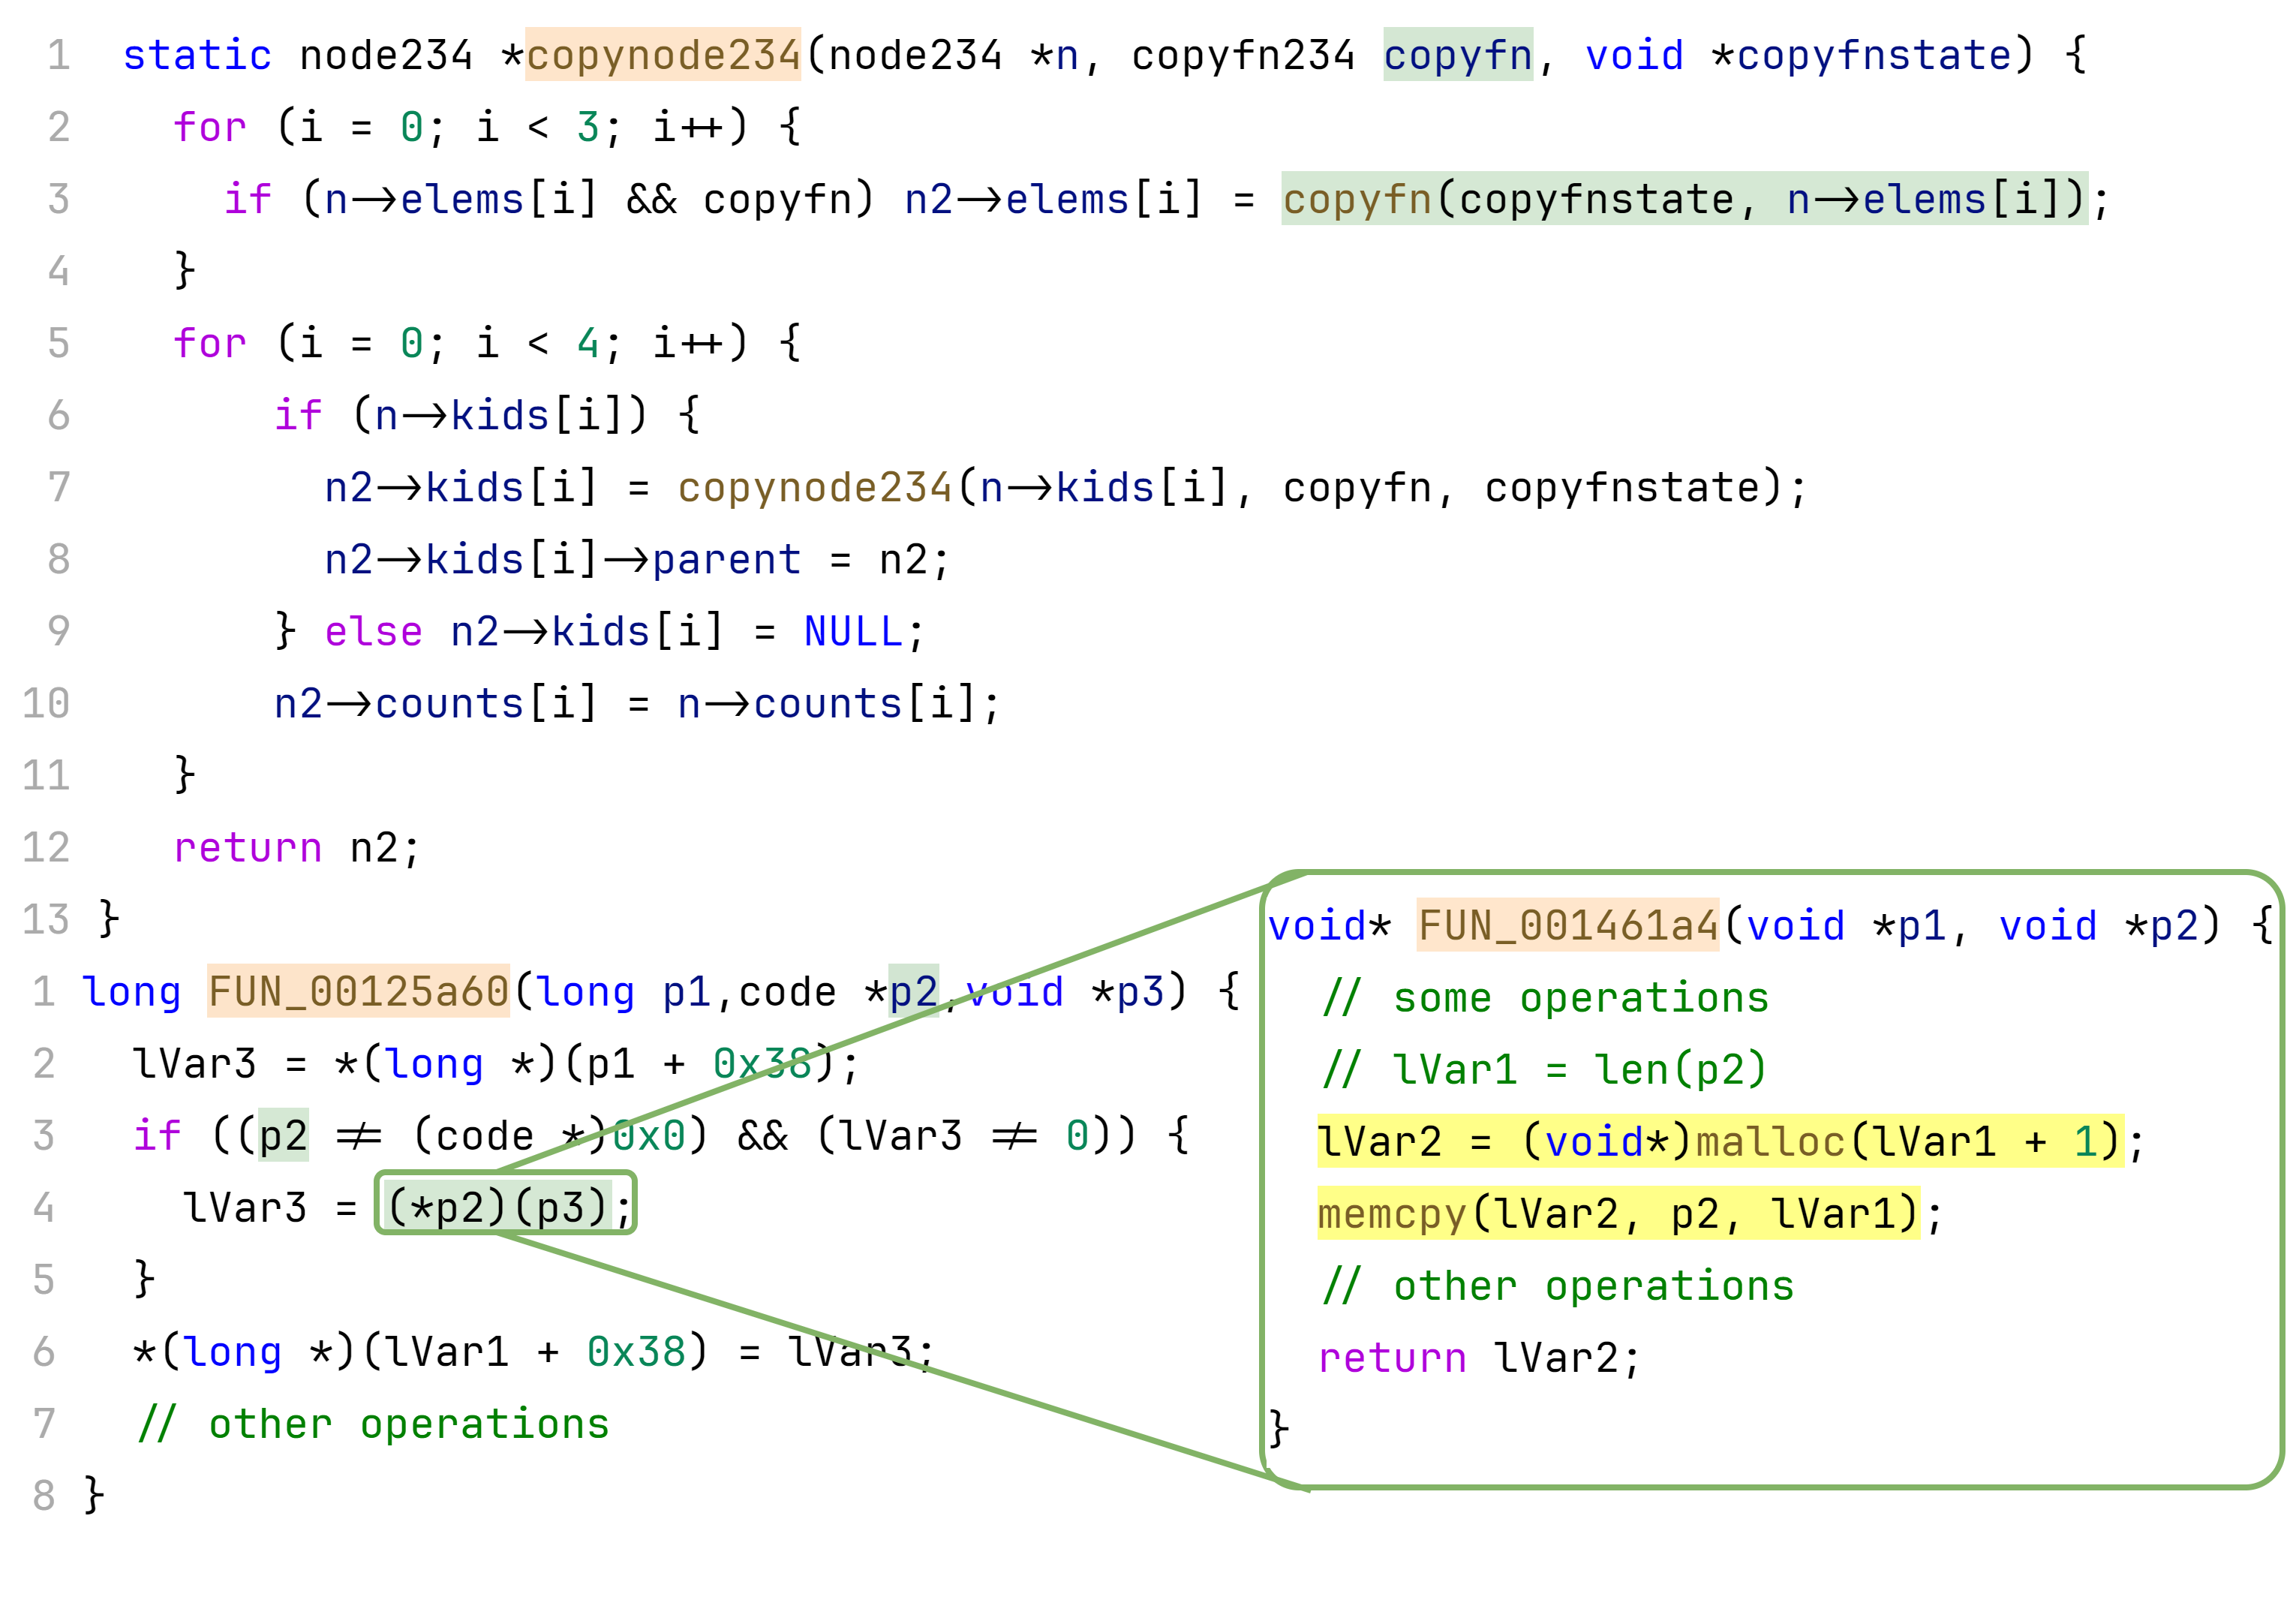
\includegraphics[width=0.8\textwidth]{img/invocation_example.drawio.png} % 调整图片宽度为文本宽度的50%
    \caption{Overview of xxx } % 添加图片标题
    \label{fig:invocation_example} % 设置图片标签,方便引用
\end{figure}

A more profound challenge stems from the prevalence of indirect and dynamic invocation mechanisms in C/C++, such as function pointers and virtual function tables. These constructs introduce substantial ambiguity into the call graph, rendering the resolution of call targets infeasible through static analysis alone. As a result, accurately reconstructing function semantics and relationships in such environments remains an open and pressing problem. \lstinline{FUN_00125a60} in Figure \ref{fig:invocation_example} is the decompiled counterpart of copynode234. The call to the copyfn function corresponds to \lstinline{(*param_2)(param_3)} on line 5. Since the target of this call depends on the value of \lstinline{param_2}, its actual destination cannot be determined by purely static analysis. This ambiguity obstructs the understanding of the callee's semantics, impeding the recovery of \lstinline{FUN_00125a60}.

Taking SymGen\cite{SymGen} as an example, we observed that many of its predicted names were placeholders like \lstinline{FUN_xxxxxx}. A closer analysis revealed that this often occurs when the primary logic of a target function A is implemented by calling another function B. Because B's name has been stripped and replaced with a placeholder, the predicted name for A inherits this placeholder. While some methods like SymLM\cite{SymLM} and NERO\cite{NERO} have attempted to model call context information, their performance has been suboptimal. We argue that this is primarily because they fail to account for the topological dependency in the call graph; that is, the logic of copynode234 can be accurately inferred only after the logic of copyfn has been determined.

\begin{minipage}[t]{0.45\textwidth}
\centering
% \renewcommand{\baselinestretch}{1.25}
\begin{lstlisting}[caption={copynode234}, basicstyle=\ttfamily\scriptsize,
keywordstyle=\color{magenta}\bfseries\scriptsize,
commentstyle=\color{Green}\itshape\scriptsize]
static node234 *copynode234(
    node234 *n, copyfn234 copyfn,
    void *copyfnstate) {
  for (i = 0; i < 3; i++) {
    if (n->elems[i] && copyfn)
      n2->elems[i] = copyfn(copyfnstate, n->elems[i]);
  }
  for (i = 0; i < 4; i++) {
    if (n->kids[i]) {
      n2->kids[i] = copynode234(n->kids[i], copyfn, copyfnstate);
      n2->kids[i]->parent = n2;
    } else n2->kids[i] = NULL;
    n2->counts[i] = n->counts[i];
  }
  return n2;
}
\end{lstlisting}
\end{minipage}
\vspace{0.3em}
\hfill
\begin{minipage}[t]{0.45\textwidth}
\centering
% \renewcommand{\baselinestretch}{1.25}
\begin{lstlisting}[caption={Pseudocode of copynode234}, basicstyle=\ttfamily\scriptsize,
keywordstyle=\color{magenta}\bfseries\scriptsize,
commentstyle=\color{teal}\itshape\scriptsize]
long FUN_00125a60(long param_1,
    code *param_2,
    undefined8 param_3){
  lVar3 = *(long *)(param_1 + 0x38);
  if ((param_2 != (code *)0x0) && (lVar3 != 0)) {
    lVar3 = (*param_2)(param_3);
  }
  *(long *)(lVar1 + 0x38) = lVar3;
  // other operations
}
\end{lstlisting}
\end{minipage}
% \renewcommand{\baselinestretch}{1.0}
\vspace{0.1em}

\textbf{Challenge 3: Unpredictable Run-time Behavior.}
We contend that static code analysis alone is insufficient for a complete understanding of program logic, especially when the code involves dynamic behaviors influenced by runtime parameters or external environment variables. This holds true even for source-level code comprehension, although the rich semantic information available in source code often mitigates its impact. In the context of stripped binaries, the effect of dynamic behavior becomes far more pronounced. This challenge is further exacerbated by modern compilers, which extensively employ optimization techniques that obscure the code's true behavior, making it exceedingly difficult to grasp its logic from a static view\cite{sig_meet_opt}.

Consider a function \lstinline{ParseNanos} from a real-world project (RTranslator) and its decompiled variant, shown in Figures~\ref{fig:dynamic_example} (a) and (b), respectively. The function accepts string pointer data, writes the parsed nanosecond value to the output parameter \lstinline{nanos}, and returns the new position of the data pointer. Its core logic, a loop spanning lines 4-8, extracts digits from the string and stores them in value. Lines 9-12 pad the number with zeros if it has fewer than 9 digits, and the final result is output on lines 13 and 14. The source code is readily understandable. However, after compilation with optimizations (-O2), its decompiled representation exhibits altered logical expressions, although the functionality remains equivalent. For example, the original condition "parse at most 9 characters" is transformed into \lstinline{if(8 < uVar3)}. As shown in Table~\ref{tab:dynamic_example}, this transformation not only increases the difficulty of semantic understanding but can also mislead predictions of models.

\begin{figure}[h] % [h] 表示图片放置在当前位置
    \centering
    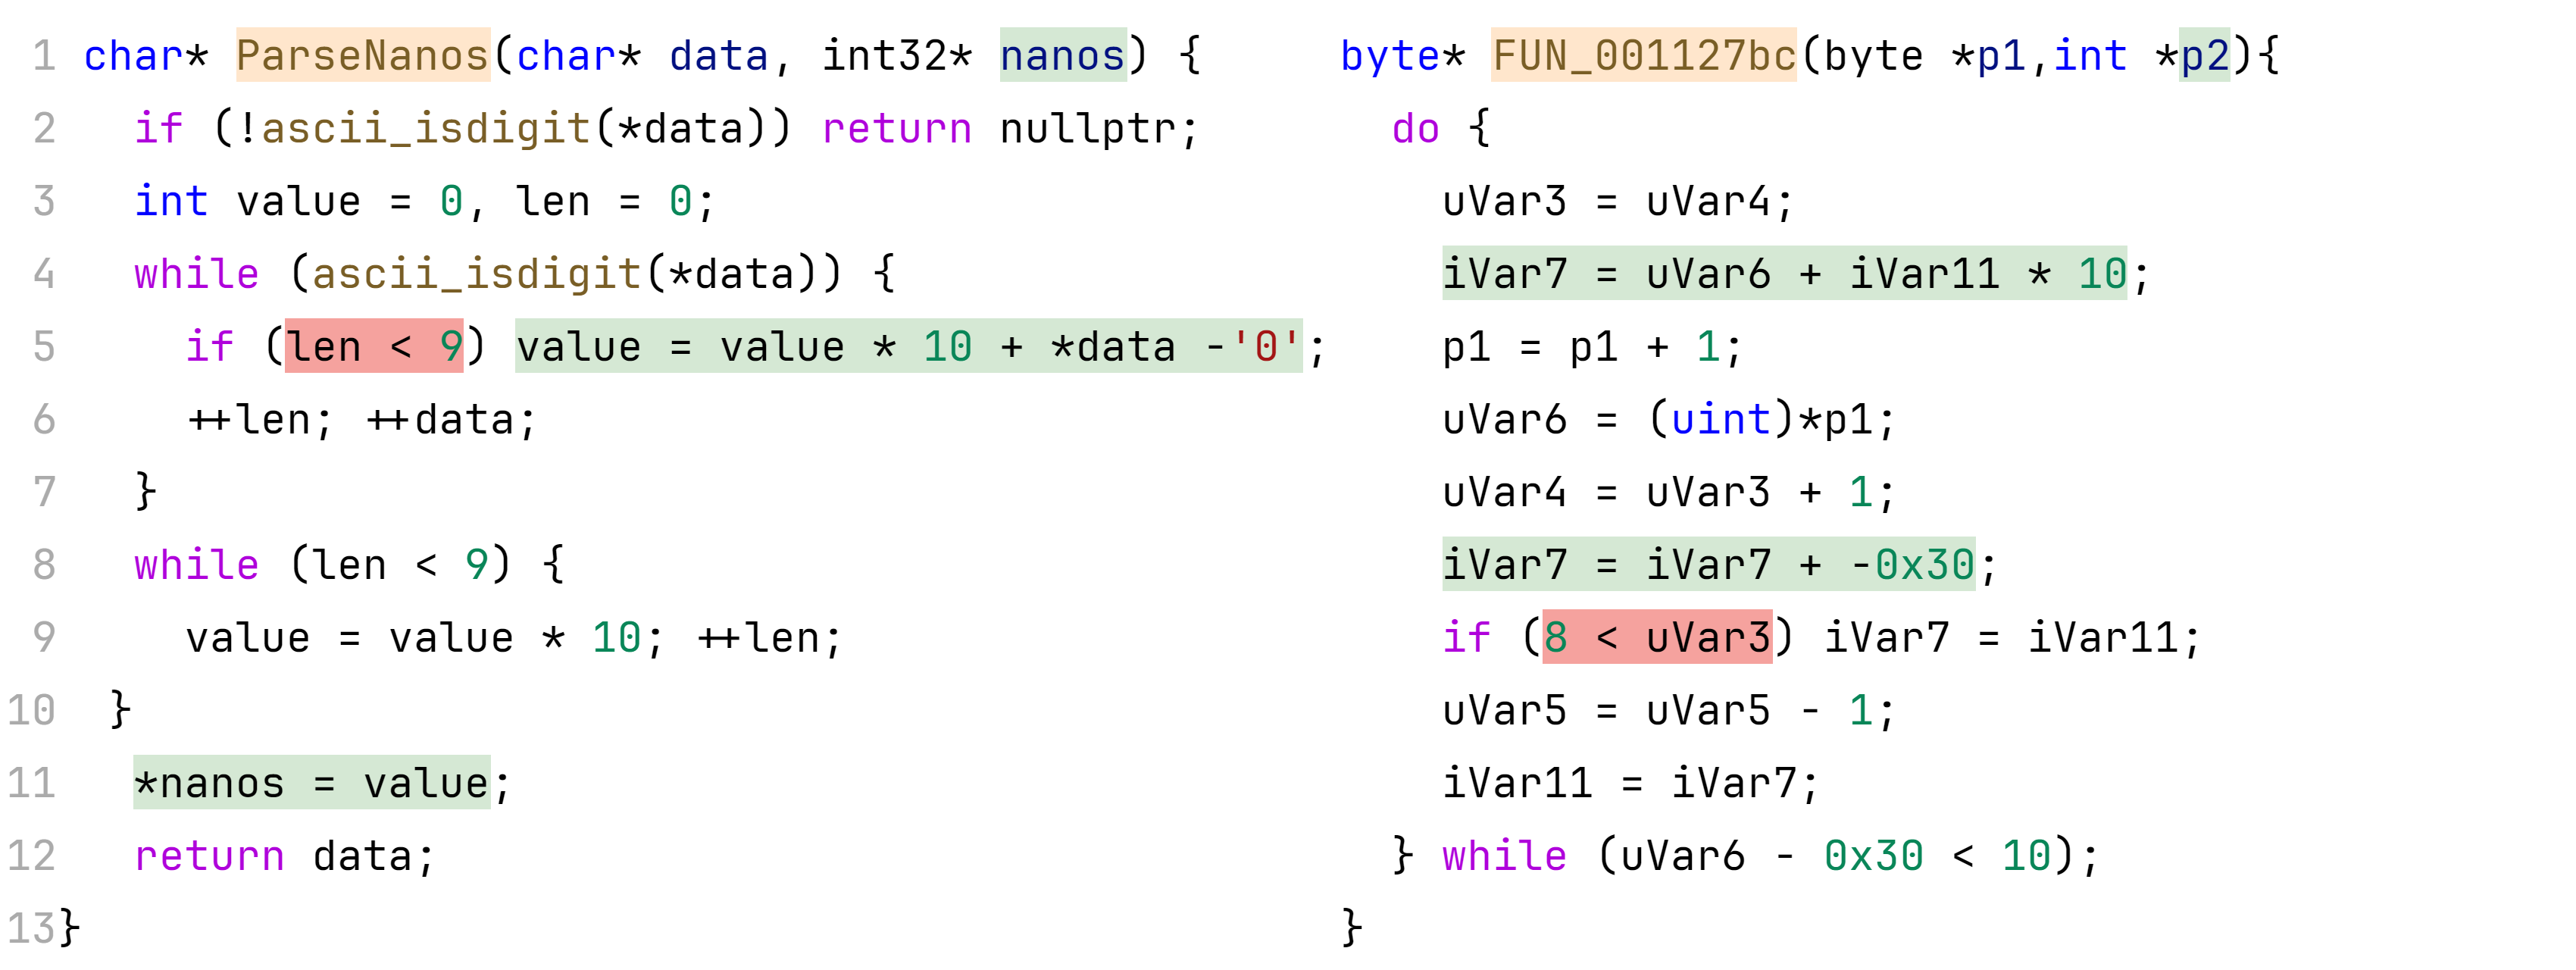
\includegraphics[width=0.8\textwidth]{img/dynamic_example.drawio.png} % 调整图片宽度为文本宽度的50%
    \caption{Overview of xxx } % 添加图片标题
    \label{fig:dynamic_example} % 设置图片标签,方便引用
\end{figure}

\begin{minipage}[t]{0.45\textwidth}
%\noindent
\begin{lstlisting}[caption={ParseNanos},
basicstyle=\ttfamily\scriptsize,
keywordstyle=\color{magenta}\bfseries\scriptsize,
commentstyle=\color{teal}\itshape\scriptsize]
const char* ParseNanos(const char* data, int32* nanos) {
  if (!ascii_isdigit(*data)) return nullptr;
  int value = 0, len = 0;
  while (ascii_isdigit(*data)) {
    if (len < 9) value = value * 10 + *data - '0';
    ++len;
    ++data;
  }
  while (len < 9) {
    value = value * 10;
    ++len;
  }
  *nanos = value;
  return data;
}
\end{lstlisting}
\end{minipage}
\hfill
\begin{minipage}[t]{0.45\textwidth}
\begin{lstlisting}[caption={Decompiled counterpart of ParseNanos},
basicstyle=\ttfamily\scriptsize,
keywordstyle=\color{magenta}\bfseries\scriptsize,
commentstyle=\color{teal}\itshape\scriptsize]
byte * FUN_001127bc(byte *param_1,int *param_2){
  if (9 < *param_1 - 0x30) {
    return (byte *)0x0;
  }
  do {
    uVar3 = uVar4;
    iVar7 = uVar6 + iVar11 * 10;
    param_1 = param_1 + 1;
    uVar6 = (uint)*param_1;
    uVar4 = uVar3 + 1;
    iVar7 = iVar7 + -0x30;
    if (8 < uVar3) {
      iVar7 = iVar11;
    }
    uVar5 = uVar5 - 1;
    iVar11 = iVar7;
  } while (uVar6 - 0x30 < 10);
  // other operations
}
\end{lstlisting}
\end{minipage}

% % ### Challenges

% 虽然二进制函数名恢复任务广受关注,在该领域涌现了许多相关的方法(综述中提到的方法),它们采用不同方式利用不同的信息并分别取得了一定程度的进展。但是我们发现二进制函数名称恢复任务仍然存在如下3个挑战:

% #### C1 方法的泛用性

% 以往的研究都将二进制函数名称恢复任务建模为一个分类任务(XFL、AsmDepictor、SymLM),这意味着它们的方法建立在目标函数名(部分)存在于它们的类别集合中。但是这样的假设往往很难在现实的函数名称恢复任务中成立,虽然它们采用了不同方式缓解OOV的问题,但OOV问题仍然不可避免,特别是当被用到新数据集中时。最近的SOTA(SymGen)将函数名称恢复任务建模为一个生成任务并通过微调一个LLM来处理,并从根本上解决了OOV的问题。但是由于资源和数据集的限制,这一类方法通常选择参数量较小的模型(例如CodeLLama-34B)进行微调,这使得被预测的函数或其指定架构的变体不在微调数据集中时,方法的有效性大打折扣,这主要是因为小参数模型难以真正理解二进制代码的知识,因而难以完全将其推广到未见过的二进制函数中。而且如今日益增多的二进制代码也使得微调LLM的策略的泛用性受到一定程度的影响。
% #### C2 广泛存在的函数调用
% 现实中的程序员编写的代码中广泛存在复杂的函数调用情况,如图xxx所示,函数copynode234内部通过调用copyfn完成实际的节点复制功能,并通过递归调用自身完成遍历2-3-4树的操作。虽然在将源码编译成二进制代码时,有些短小的函数会发生函数内联,但是绝大多数的复杂的调用关系仍然会被保留下来。对于源码级的函数语义理解任务,可以通过观察被调用函数的函数名来推测其语义,但在stripped binaries中,我们丢失了绝大多数的语义信息,我们只能知道被调用函数的起始地址(例如FUN_00123456),这无疑加剧了函数理解的困难。更困难的是,C/C++代码中广泛存在间接调用的行为(例如函数指针、虚函数表等)使得我们无法在静态分析中获取其调用目标。例如图xxx表示了copynode234在编译成二进制代码后的反编译对等体,第5行的`(*param_2)(param_3)`对应了`copyfn`函数的调用,它的值取决于param_2,因而无法在纯静态分析中知道其实际指向的函数,更无法知道该函数的语义信息,因而在恢复FUN_00125a60的函数名(copynode234)时存在困难。
% 以SymGen为例,我们发现它的预测结果中存在许多`FUN_xxxxxx`,仔细分析后发现它们主要是因为目标函数A的内部的主要逻辑是通过调用另一个函数B完成的,而由于B的函数名被strip掉而被替换为`FUN_xxxxxx`,因此最终的预测名也就是这样的占位符。虽然有些方法(SymLM、NERO)考虑到了将调用上下文信息进行建模,但效果并不理想。我们认为这主要是因为他们并没有考虑这种拓扑关系,即只有确定了copyfn的逻辑,才能更准确地推测copynode234的逻辑。
% #### C3 难以预测的执行行为
% 我们强调仅通过静态代码难以完全理解代码的逻辑,特别是当代码涉及动态行为时(例如代码的逻辑收到参数、外部环境变量的影响)。这样的事实对于源码级代码理解任务同样适用,只不过源码中丰富的语义信息削弱了它的影响。但当场景转化为stripped binaries时,动态行为的影响便凸显出来了,尤其是现代编译器在将源代码编译成二进制代码时广泛使用编译优化技术,更进一步隐藏了代码的真实行为,使得我们难以仅通过静态代码准确理解代码的逻辑。
% 以图xxx和图xxx为例,它们是一个真实项目(RTranslator)中的某个函数ParseNanos的源码和对应的反编译变体。它接受一个表示字符串的指针data,并将第二个参数nanos作为解析结果输出,并返回解析后data指向的新位置。它的核心逻辑在于第4-8行的while循环,用于将data指向的字符串中的数字提取并存入value,第9-12行则是对不满足9位的数填0,最后通过13和14行输出结果。我们通过源代码很容易理解其逻辑,但是将其编译为二进制代码(并通过Ghidra反编译得到伪C代码)后,由于编译优化(-O2)的影响,它的部分逻辑表达形式发生了变化(虽然功能仍然等价)。源代码中体现“解析至多9位字符”的条件语句在反编译变体中却以`if(8 < uVar3)`的形式表达。这在一定程度上增加了语义理解的困难,甚至会误导方法的预测。例如使用SymGen、XFL和LLM预测时的这一种可能结果如表xxx所示


\begin{table}[t]
  \centering
  \footnotesize
  \caption{Influence of Run-Time Behavior}
  \label{tab:dynamic_example}
  \renewcommand\arraystretch{1.15}
\begin{tabular}{p{1.7cm}p{1.7cm}p{1.2cm}p{1.2cm}p{1.2cm}p{1.2cm}p{1.2cm}}
\toprule
patterns & sub-pattern &xx dynaic &xx static & xfl &symGen    \\
\midrule
\textbf{Method(19)} & Missing(12) &5 &1 &\textbf{9} &5 &2 \\
\textbf{Method(19)} & Noncallable(6) &5 &1 &\textbf{9} &5 &2 \\
\textbf{Return value(29)} & Noncallable(6) &\textbf{17}&\textbf{5}&0&0&7\\
\bottomrule
\end{tabular}
\end{table}


\subsection{Key Insights}

Our approach, HyBinMAS, is motivated by the need to overcome the limitations of current LLM-based methods in handling challenges such as fast-evolving codebases, OOV symbols, dynamic features and  unpredictable run-time behaviors. By leveraging a multi-agent, feedback-driven framework that integrates both static and dynamic analysis, we aim to provide a more flexible, accurate, and future-proof solution for code recovery tasks. %In recent years, LLMs have demonstrated remarkable efficacy across numerous source-level programming tasks. Pioneering research such as SymGen and FoC has illuminated their potential for understanding the semantics of binary code. We are therefore convinced that leveraging capacities of LLMs remains a promising strategy.
Specifically, HyBinMAS considers three key insights as follows:

To address \textbf{Challenge 1}, instead of fine-tuning small models like CodeLlama, HyBinMAS utilizes a general-purpose LLM as its foundational component, structured within a Multi-Agent System. It eliminates the need for meticulous fine-tuning, thereby attaining superior generalizability, considering the inherent drawbacks of fine-tuning large-scale LLMs, which is both resource-intensive and time-consuming\cite{LLaMA}.

To tackle \textbf{Challenge 2}, HyBinMAS employs a hybrid static-dynamic analysis to resolve function call graphs, which will be detailed in Section~\ref{sec:hsda_design}. Activation of this call relationship is explicitly considered during the name prediction phase. We observed that reverse engineers often adopt a recursive mindset when analyzing function calls: if function A calls function B, they typically analyze B first and use the resulting semantic understanding to inform their analysis of A. Inspired by this practice, HyBinMAS follows a similar bottom-up process. It first recovers the names of the functions called within a target function and then leverages this information to recover the name of the target function itself. Returning to the example in Figure~\ref{fig:invocation_example}, by analyzing the call relationships of \lstinline{FUN_00125a60}, we can determine the actual function pointed to by \lstinline{param_2}, deduce that its logic is related to copying, and consequently predict a more accurate name, as shown in Figure~\ref{fig:invocation_example} (b). Without this strategy, one might only discern that the function performs a recursive traversal, without knowing the specific operation being performed during the traversal.

For \textbf{Challenge 3}, HyBinMAS first seeks to emulate the human thought process as an experienced reverse engineer not only "reads" the code but also "runs" it. After forming an initial hypothesis about the code's semantics through static inspection, they will construct test cases to execute the function and observe its dynamic behavior. This allows them to validate or refute their initial assumptions and guide further analysis. We believe this is a highly effective method for addressing the challenge. For the function \lstinline{ParseNanos}, the initial LLM predictions in Table~\ref{tab:dynamic_example} were semantically close but incorrect regarding the precise number of digits, which is a fitting example of being misled by compilation optimizations. Based on the initial semantic hypothesis, HyBinMAS generates the test cases shown in "HyBinMAS-S" column of Table~\ref{tab:dynamic_example}. Upon execution, it observes that for test case 4, which expects only the first 8 characters to be parsed, all 9 digits are actually processed. This execution trace is summarized into a feedback report that directs the LLM to revise its previous inference. Through several iterations of this process, HyBinMAS arrives at the more accurate semantic prediction shown in the "HyBinMAS" column of Table~\ref{tab:dynamic_example}.

Furthermore, we acknowledge that not all functions can be executed successfully. A more complex example is presented in Figure xxx (see Appendix for decompiled code). The LLM's initial semantic interpretation was simply \lstinline{remove}, a description that is clearly imprecise. However, because this function takes a pointer to a custom structure as a parameter, attempts to generate test cases and execute it frequently lead to illegal memory access and program crashes. HyBinMAS addresses this by using an additional LLM to summarize the generated test cases and the execution failure logs into a new feedback report. By providing this consolidated feedback to the primary LLM, HyBinMAS facilitates a more accurate prediction: \lstinline{remove_env}.

% % ### Motivation

% 近年来,LLM已经在许多源码级任务上展现出非凡的有效性,以SymGen、FoC为代表的研究也让我们看到了LLM在理解二进制代码语义上的潜力,因此我们相信LLM在理解二进制代码语义上仍然是一种有效的策略。为了解决C1的问题,我们不对小参数模型(如CodeLlama)进行微调,而是选择使用较大参数的通用LLM作为基础组件,并将其搭建成一个Multi-Agent系统。在这种策略下我们不再需要精心微调LLM,这在一定程度上实现了更强的泛用性效果(微调大参数模型及其消耗资源与时间)。

% 为了解决C2,HyBinMAS会首先处理目标so文件,并通过动静态混合分析的方式确定函数调用关系,并在预测函数名时显示考虑这样的调用关系。我们观察到逆向工程师通常采用递归的思想处理函数调用:即如果FUN_A调用了FUN_B,那么他们会先分析FUN_B,并将FUN_B的语义理解结果提供给FUN_A。受到这一事实的启发,HyBinMAS在恢复函数名时也会进行相似的过程:先对目标函数的函数中调用的函数进行名称恢复,再利用得到的信息完成对目标函数的名称恢复。以图xxx为例,通过分析FUN_00125a60的调用关系,我们可以确定param_2实际指向的函数,并分析出它的逻辑与copy相关,据此推测出了如图xxx所示的更准确的答案。如果没有这样的策略,我们只能知道该函数在进行一个递归遍历操作,而不知道它在遍历执行什么具体的操作。

% 我们观察到一名资深的逆向工程师不只会“看”代码,还会“跑”代码。他们通过“看”代码初步理解其语义信息后,会尝试构造一些测试样例,并执行目标函数,观察其动态行为是否与自己之前的推测一致,据此进行下一步的理解,我们认为这正是解决C3的一种有效方法。以ParseNanos函数为例,我们看到表xxx中LLM的预测结果基本吻合,但是在关键的位数中出现了错误,它正是被编译优化的结果误导了。根据其语义信息,为期提供表xxx所示的测试样例并执行,我们发现测试样例4期望只提取前8个字符,但是实际上9个字符均完整地得到了。这样的执行信息会被总结成了反馈信息指导LLM修正前一轮的推测结果。这一过程将迭代多轮,最终预测出了表xxx HyBinMAS列所示的更准确的语义信息。

% 另外,我们强调并不是所有函数都能够被正确地执行。图xxx是一个更为复杂的例子(反编译代码见附录)。LLM初次语义理解的结果为`remove`,这样的结果显然不够准确。但因为它有一个自定义结构体指针的参数,因此在生成测试样例并执行时很容易出现非法访问而导致程序异常退出的情况。通过利用额外的LLM将测试样例和执行失败的日志信息总结成反馈信息并提供给LLM,HyBinMAS实现了更为准确的推测结果`remove_env`。

% In conclusion, xxx

\section{Method Design}
% \begin{figure}[h] % [h] 表示图片放置在当前位置
%     \centering
%     \includegraphics[width=0.5\textwidth]{image/ConstructDataset.drawio.png} % 调整图片宽度为文本宽度的50%
%     \caption{An overview of the dataset construction process} % 添加图片标题
%     \label{fig:construct-dataset} % 设置图片标签,方便引用
% \end{figure}
\begin{figure}[h] % [h] 表示图片放置在当前位置
    \centering
    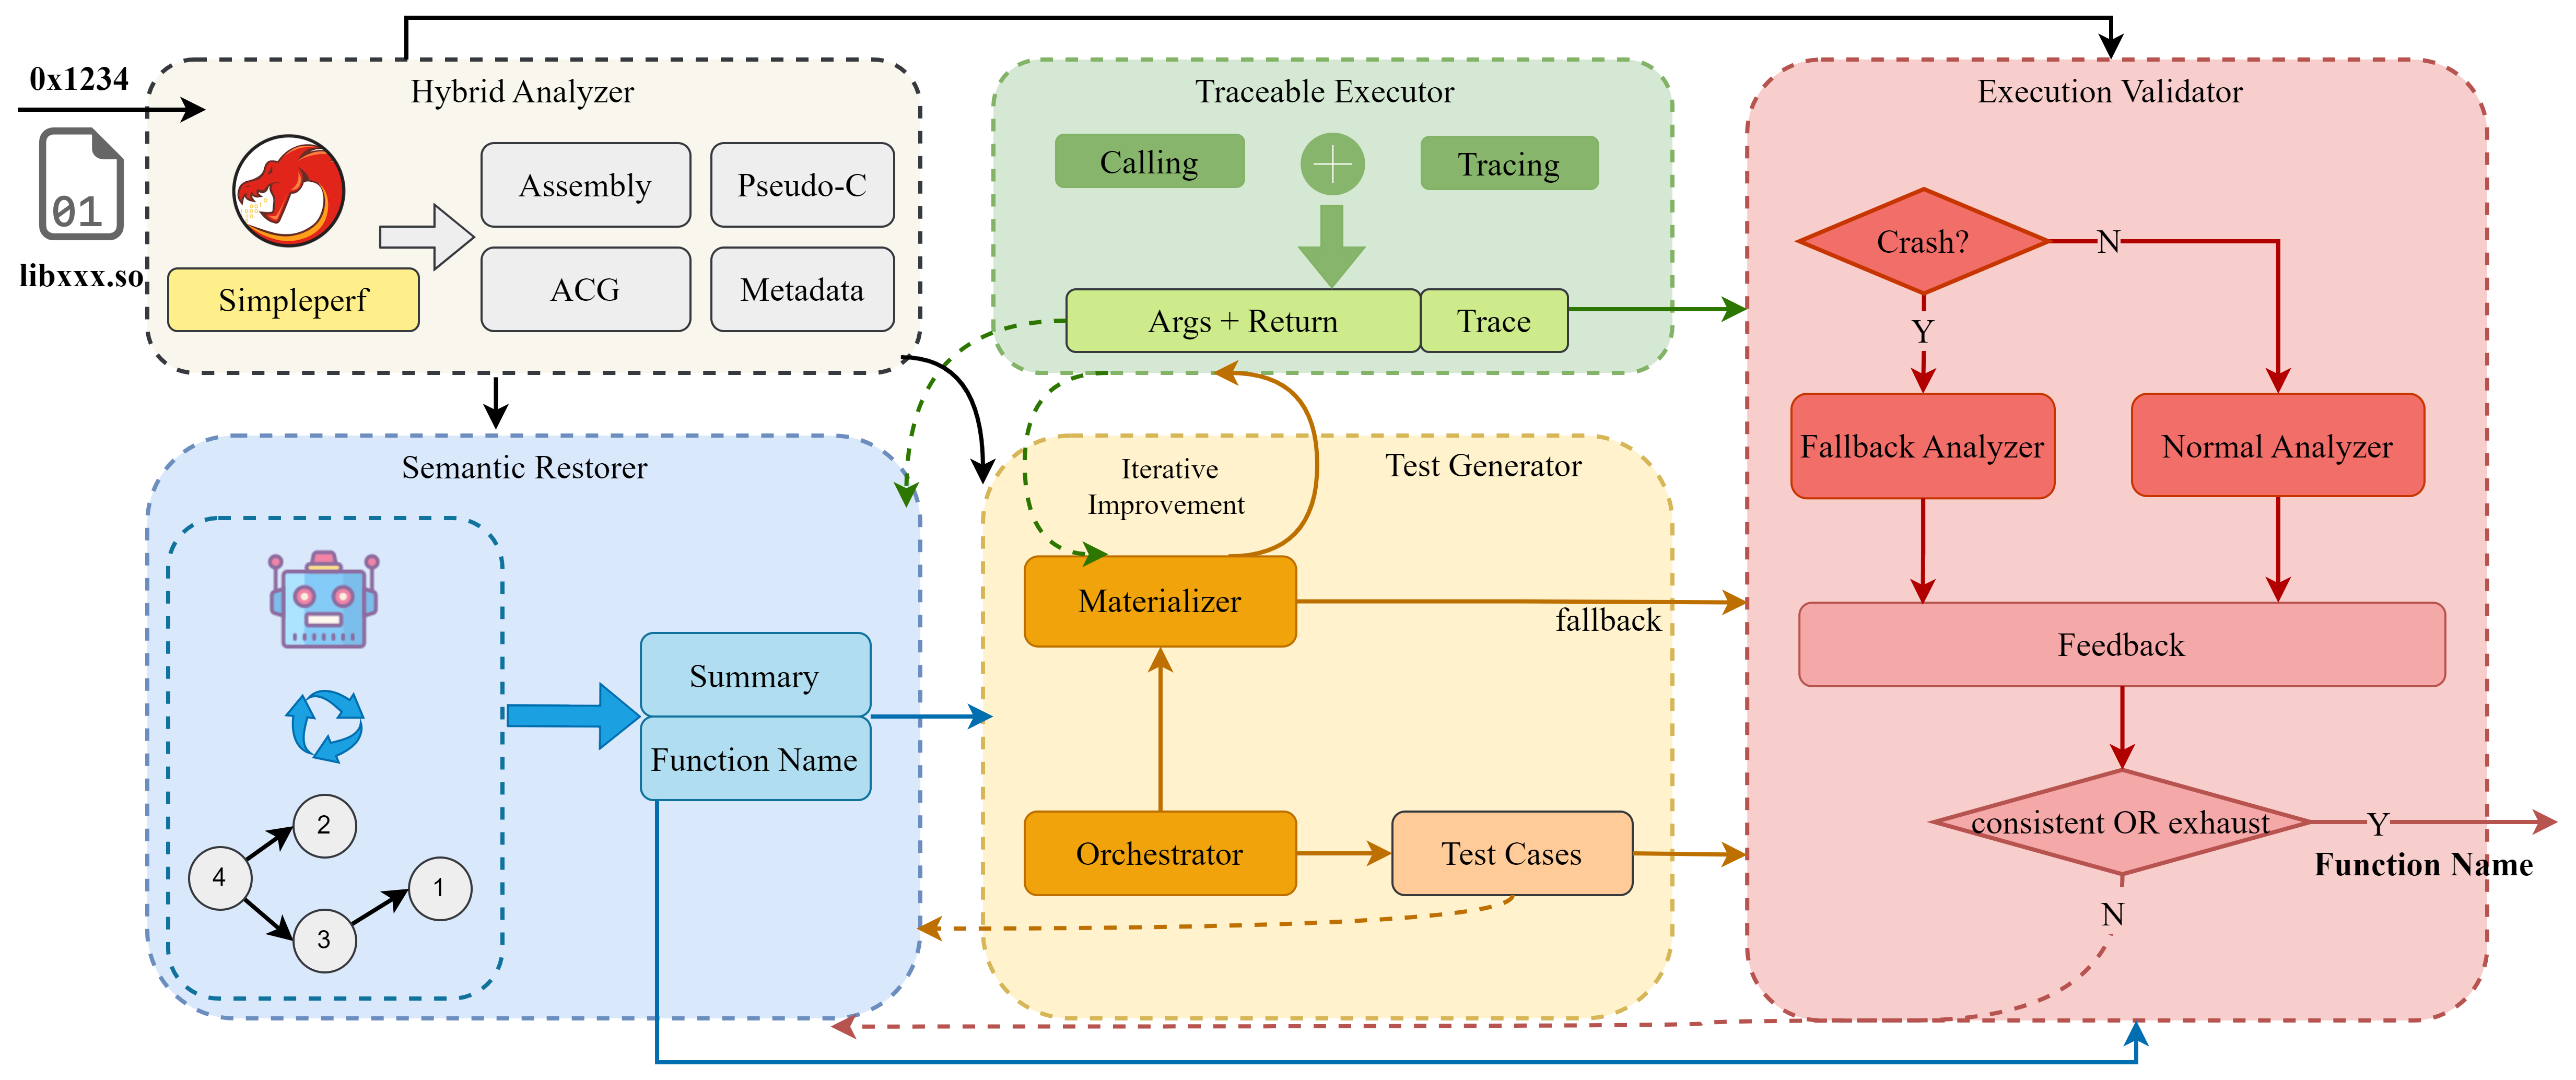
\includegraphics[width=0.8\textwidth]{img/Overview.drawio.png} % 调整图片宽度为文本宽度的50%
    \caption{Overview of xxx } % 添加图片标题
    \label{fig:overview} % 设置图片标签,方便引用
\end{figure}

\subsection{Overview}
Inspired by the process human experts employ to manually comprehend the semantics of stripped functions and recover their names, we introduce \textbf{HyBinMAS}, a novel framework for binary function name recovery based on hybrid analysis and a Multi-Agent system, to address \textbf{Challange 2}. HyBinMAS identifies critical information integral to the function name recovery workflow and distills it into two fundamental services: the \textbf{HyBrid Static-and-Dynamic Analyzer (HSDA)} and the \textbf{Executor}. To fully leverage this information, HyBinMAS conceptualizes the recovery process into three crucial phases, each implemented by a dedicated Agent: the \textbf{Semantic Restorer (SR)}, the \textbf{Test Generator (TG)}, and the \textbf{Execution Validator (EV)}. To maximize the synergistic potential of these Agents and enhance the accuracy of the final name prediction, we have meticulously orchestrated their collaboration within the workflow depicted in Figure \ref{fig:overview}. Furthermore, Algorithm \ref{alg:HyBinMAS} precisely delineates the interplay between these Agents and the fundamental services.
\begin{figure}[h] % [h] 表示图片放置在当前位置
    \centering
    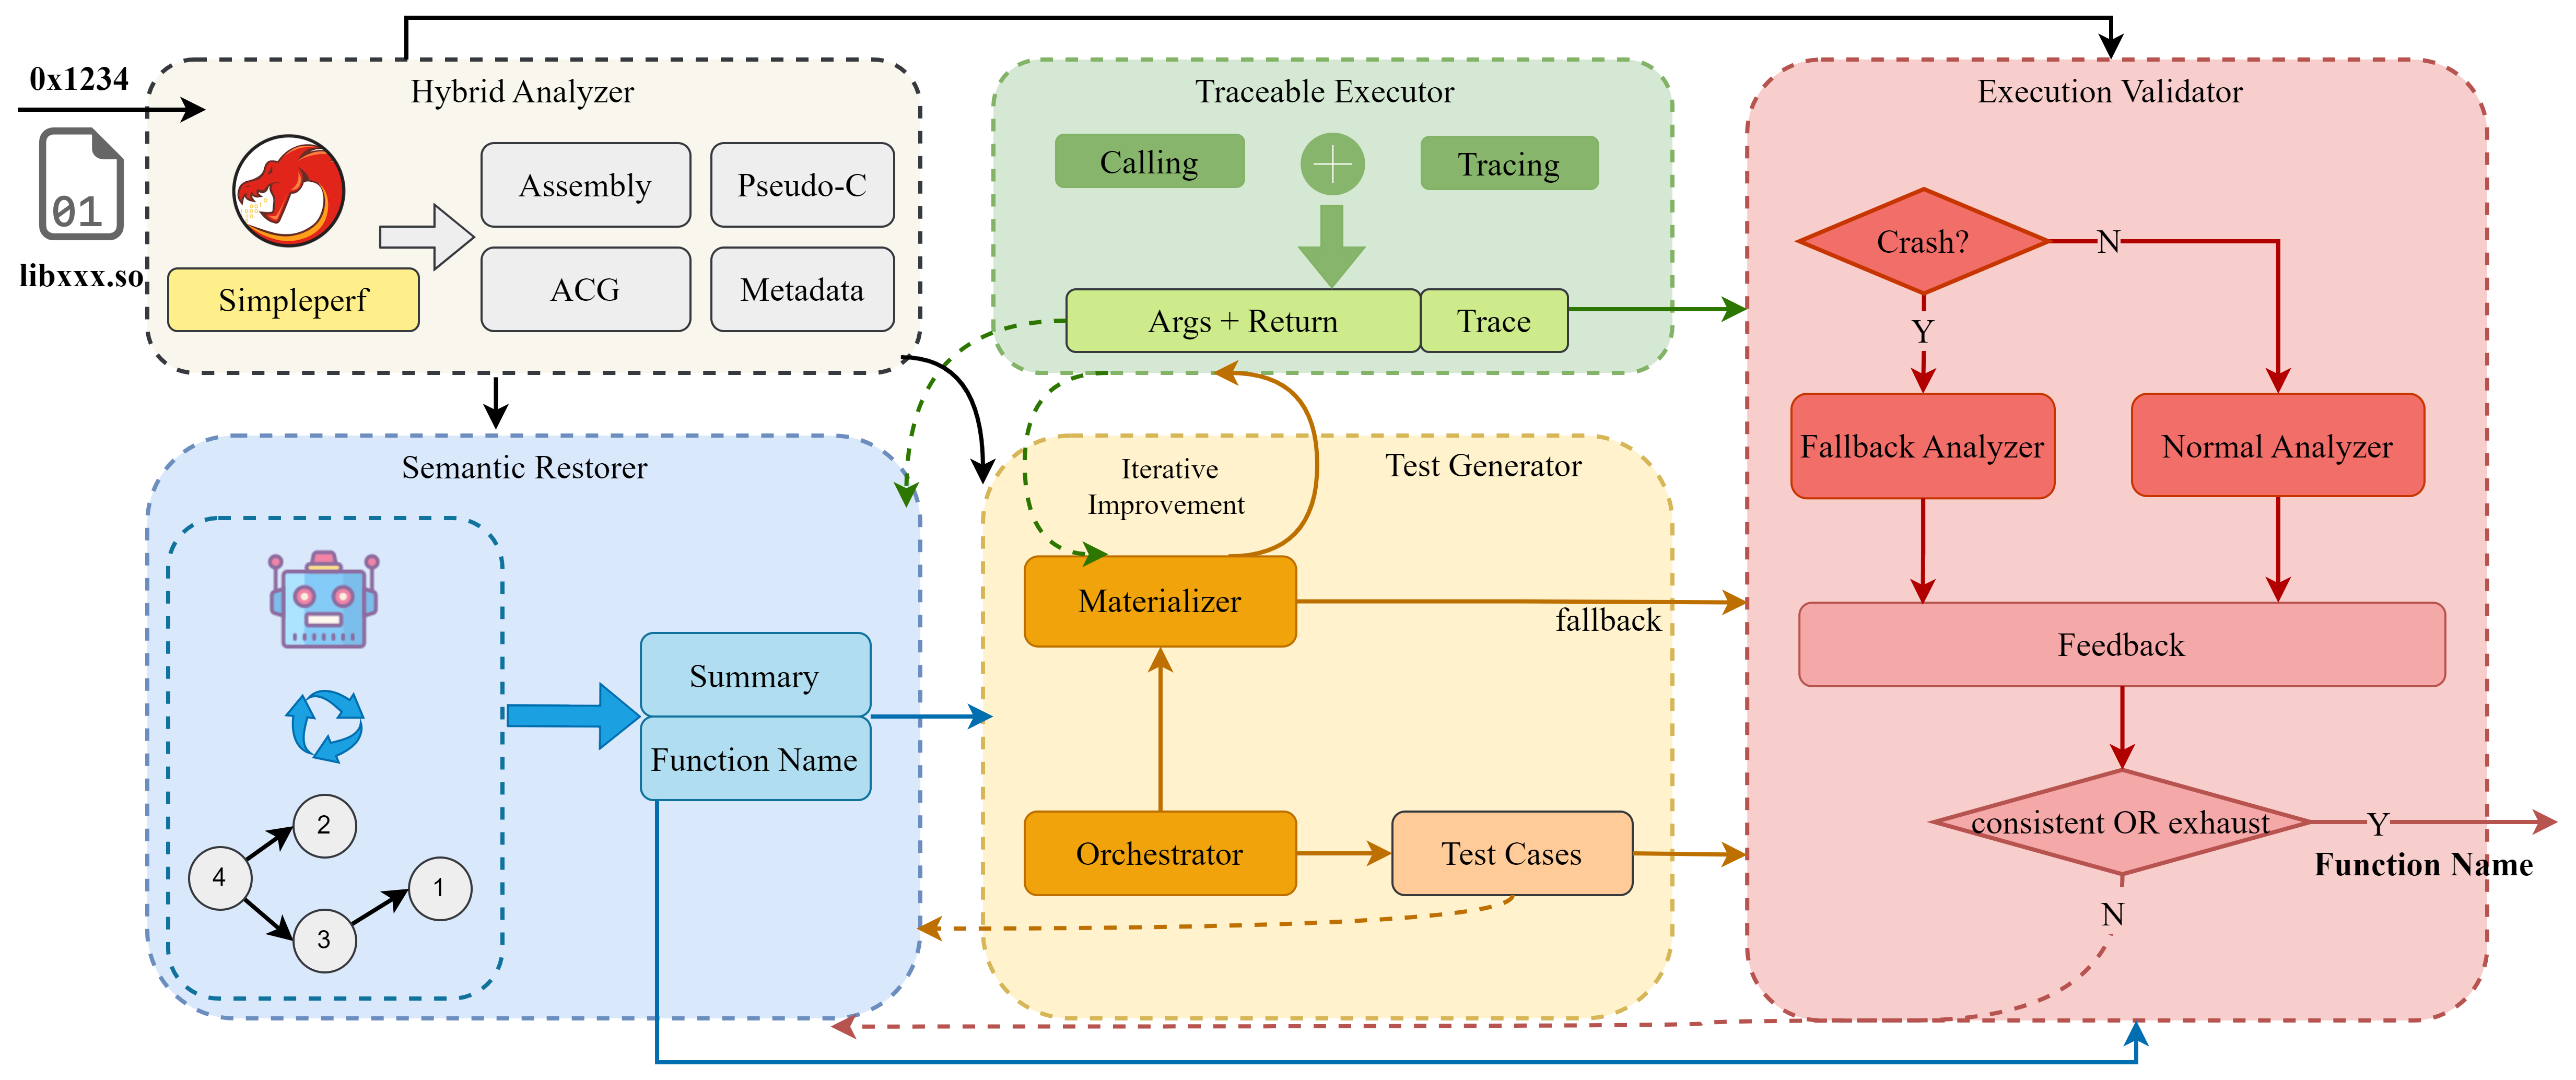
\includegraphics[width=0.5\textwidth]{img/Overview.drawio.png} % 调整图片宽度为文本宽度的50%
    \caption{Overview of the HyBinMAS} % 添加图片标题
    \label{fig:overview} % 设置图片标签,方便引用
\end{figure}
\begin{algorithm}
  \caption{Consensus-Guided Function Naming Algorithm}
  \label{alg:HyBinMAS}
  \begin{algorithmic}[1]
    \REQUIRE $o$: The offset of target function, $B$: The binary containing target function, $metadata$: The metadata of $B$, $M$: The maximum iterations, $R$: The maximum retries for execution failure, $K$: The maximum numbers of test cases
    \ENSURE $l$: The predicted function name

    \STATE $\langle a, p, \mathcal{ACG}_o, metadata \rangle \gets \text{HSDA}(o, B)$
    \STATE $\langle l, s \rangle \gets \text{SR}(\mathcal{ACG}_o, o, A, P, M, metadata, \text{NULL})$ \textit{// without feedback}
    \FOR{$m \gets 1$ \textbf{to} $M$}
        \STATE $T \gets \text{TG}(l, s, p, K)$
        \STATE $F \gets \varnothing$
        \FORALL{$t \in T$}
            \STATE $\langle err, args, ret, trace \rangle \gets \text{Executor}(t, R)$
            \IF{$err \ne \text{NULL}$}
                \STATE $f \gets \text{FallbackAnalyer}(t, err)$
            \ELSE
                \STATE $f \gets \text{NormalAnalyzer}(t, args, ret, trace)$
            \ENDIF
            \STATE $F = F \cup f $
        \ENDFOR
        \STATE $feedback \gets \texttt{generate\_feedback}(F)$
        \IF{$\texttt{check\_consistent}(feedback)$}
            \RETURN $l$
        \ENDIF
        \STATE $\langle l, s \rangle \gets \text{SR}(\mathcal{ACG}_o, o, a, p, M, metadata, feedback)$ \textit{// with dynamic feedback}
    \ENDFOR
    \RETURN $l$
  \end{algorithmic}
\end{algorithm}

The process is initiated by providing HyBinMAS with its inputs: the binary file, control parameters outlined in Algorithm \ref{alg:HyBinMAS}, and a target function uniquely identified by its offset. The process then unfolds as follows: \textbf{(\textit{i})} The \textbf{HSDA} performs a hybrid static-dynamic analysis on the target function and its containing binary file, yielding the function's assembly code $a$, decompiled code $p$, Attributed Call Graph $\mathcal{ACG}$, and other pertinent metadata (Line 1 of Algorithm \ref{alg:HyBinMAS}). \textbf{(\textit{ii})} The \textbf{SR} leverages this comprehensive information to generate an initial predicted function name $l$ and a semantic summary $s$ (Line 2 of Algorithm \ref{alg:HyBinMAS}). \textbf{(\textit{iii})} Subsequently, the \textbf{TG} synthesizes a suite of suitable test cases $T$ based on the decompiled code from the HSDA and the name and summary provided by the SR (Line 4 of Algorithm \ref{alg:HyBinMAS}). \textbf{(\textit{iv})} The \textbf{Executor} then proceeds to run each test case generated by the TG, capturing both the execution data and any error information. \textbf{(\textit{v})} Finally, the \textbf{EV} analyzes the outcome of each execution. Depending on whether a test case succeeded or failed, it selects an appropriate analyzer to process the results, summarize the collective execution feedback from the entire test suite and replay it to the SR for refinement and improvement.

% 受到人工理解Stripped functions语义信息并恢复其函数名的一般流程的启发,我们提出了一个基于混合分析和Multi-Agent的二进制函数名称恢复框架——HyBinMAS。HyBinMAS洞察了函数名称恢复流程中用到的重要信息并将其抽象为两个基本服务:HyBrid Static-and-JDynamic Analyzer (HSDA)和Executor。为了充分利用这些信息,HyBinMAS建模了三个重要环节,并设计了对应的Agent实现他们:Semantic Restorer(SR)、Test Generator(TG)和Execution Validator(EV)。为了能够最大程度地发挥不同Agent的能力以提升最终函数名预测的小小果,我们按照图xxx所示的工作流精心将它们组织在一起。算法xxx则准确地描述了不同Agent和服务之间的交互关系。

% 对于一个待分析的函数,可以使用它相对于二进制文件的起始偏移地址唯一标识,HyBinMAS将该函数和所在的二进制文件作为输入(以及算法xxx所示的控制算法流程的必要参数)。(1)HSDA对目标二进制函数和so文件进行动静态混合分析,并得到目标函数的反汇编代码、反编译代码、调用图和其他元信息(算法xxx中的第1行)。(2)SR充分利用这些信息,生成预测的函数名和摘要(算法xxx中的第2行)。(3)TG根据HSDA输出的反编译代码和SR输出的函数名和摘要生成合适的测试样例集(算法xxx第4行)。(4)Executor逐个执行TG生成的测试样例,并获取执行信息和错误信息。(5)EV逐个分析Executor的执行结果,根据是否执行成功选择合适的分析器进行分析,总结测试样例集的执行信息并反馈给SR进行修正与改进。如算法xxx所示,HyBinMAS至少执行一次SR分析静态信息,并在第6-19行通过迭代至多M次步骤(3)(4)(5)(2)来修正第一次SR输出的语义信息。接下来我们会讨论每一步骤的细节。

As illustrated by Algorithm \ref{alg:HyBinMAS}, HyBinMAS performs at least one initial static analysis pass with the SR. This is followed by an iterative refinement loop (Lines 6-19), which repeats steps \textbf{(\textit{iii})}, \textbf{(\textit{iv})}, \textbf{(\textit{v})} and \textbf{(\textit{ii})} for up to $M$ iterations to progressively improve the initial semantic inference of SR. In the following sections, we will elaborate on the details of each step.



\subsection{Hybrid Static-and-Dynamic Analyzer Service}
\label{sec:hsda_design}

As the inaugural component of the \textbf{HyBinMAS} framework, the \textbf{Hybrid Static-and-Dynamic Analyzer (HSDA)} accepts a target function (e.g., \texttt{+0x1234}) and its containing binary(e.g., \texttt{libxxx.so}) as initial inputs to perform a hybrid static-dynamic analysis. Given that the HSDA serves as a foundational service, its output provides the essential basis for all subsequent stages. Existing research\cite{SymGen}has demonstrated that decompiled code contributes more significantly to semantic comprehension than raw assembly code. Therefore, we designate the decompiled pseudo-code as a primary output of the HSDA module for downstream use. Building upon this foundation, the HSDA incorporates the following key advancements:

We recognize that such decompiled code does not strictly represent the actual execution order. In contrast, assembly code maintains a high degree of fidelity with the sequence of executed instructions. Consequently, we designed the HSDA to also output the assembly code, which is specifically utilized by the downstream Execution Validator (EV). Furthermore, the HSDA is leveraged to extract the function's signature, encompassing the types and storage locations (e.g., registers or stack offsets) of its parameters and return value. This signature information not only provides fundamental support for the Semantic Restorer's (SR) inference process but also serves as a critical prerequisite for generating and executing test cases.

To address \textbf{Challange 2}, we posit that a comprehensive understanding of function call context is indispensable for semantic analysis. The prevalence of indirect calls in C/C++ (as exemplified in Figure~\ref{fig:invocation_example}) renders static analysis alone insufficient to construct a complete call graph, which, in turn, impairs the performance of name recovery. We therefore begin by defining a formal data structure, the \textbf{Attributed Call Graph (ACG)}, denoted as \( \mathcal{ACG} = (\mathcal{V}, \mathcal{E}) \). The vertex set, \(\mathcal{V} \subseteq \mathcal{N} \times \mathcal{L} \times \mathcal{S}\), consists of tuples \(v = (n, l, s)\), where \(\mathcal{N}\) is the set of unique function identifiers, \(\mathcal{L}\) is the space of predicted function names, and \(\mathcal{S}\) is the space of summaries. The edge set, \(\mathcal{E} = \mathcal{E}_{s} \cup \mathcal{E}_{d}\), represents the union of static and dynamic calls. An edge \(e \in \mathcal{E}\) is a tuple \((n_u, n_v, cs, exp_{cs})\), where \(n_u\) is the caller, \(n_v\) is the callee, \(cs\) is the call site address, and \(exp_{cs}\) is the corresponding call expression in the decompiled code.

The process begins with an initial $\mathcal{ACG}$ derived from static analysis tools, as depicted in Figure~\ref{fig:acg_transform} \normalsize{\textcircled{\scriptsize{I}}}\normalsize. This initial graph is partially attributed to vertices that lack semantic information (names and summaries) and fully attributed static edges, \(\mathcal{E}_s\). The enrichment of vertex attributes is a core responsibility of the SR component, which will be detailed in Section~\ref{sec:sr_design}. To populate the dynamic edge set \(\mathcal{E}_d\), we first capture dynamic call traces as a set of pairs $\langle cs, ct \rangle$, where \(cs \in \mathcal{CS}\) is a call site and \(ct \in \mathcal{N}\) is its dynamically resolved target. We then formalize the augmentation process with the following definition for \(\mathcal{E}_d\):
\begin{equation}
\label{eq:dynamic_augment}
\mathcal{E}_d = \{ (n_u, ct, cs, exp_{cs}\}) \mid n_u \in \mathcal{N} \land cs \in \text{Sites}(n_u) \land \langle cs, ct \rangle \text{ is an observed dynamic call} \}
\end{equation}
In Equation~\ref{eq:dynamic_augment}, \(\text{Sites}(n_u)\) denotes the set of all call sites within function \(n_u\), and \(exp_{cs}\) is the decompiled expression aligned with the call site \(cs\).

This augmentation process is visually depicted in grey arrows of Figure~\ref{fig:acg_transform}. Initially, the ACG contains only the static call relationships (e.g., between functions A, B, and D). By applying the rule of Equation~\ref{eq:dynamic_augment}, we enrich the graph with the newly discovered dynamic call edges, represented by the dashed arrows.

\begin{figure}[h] % [h] 表示图片放置在当前位置
    \centering
    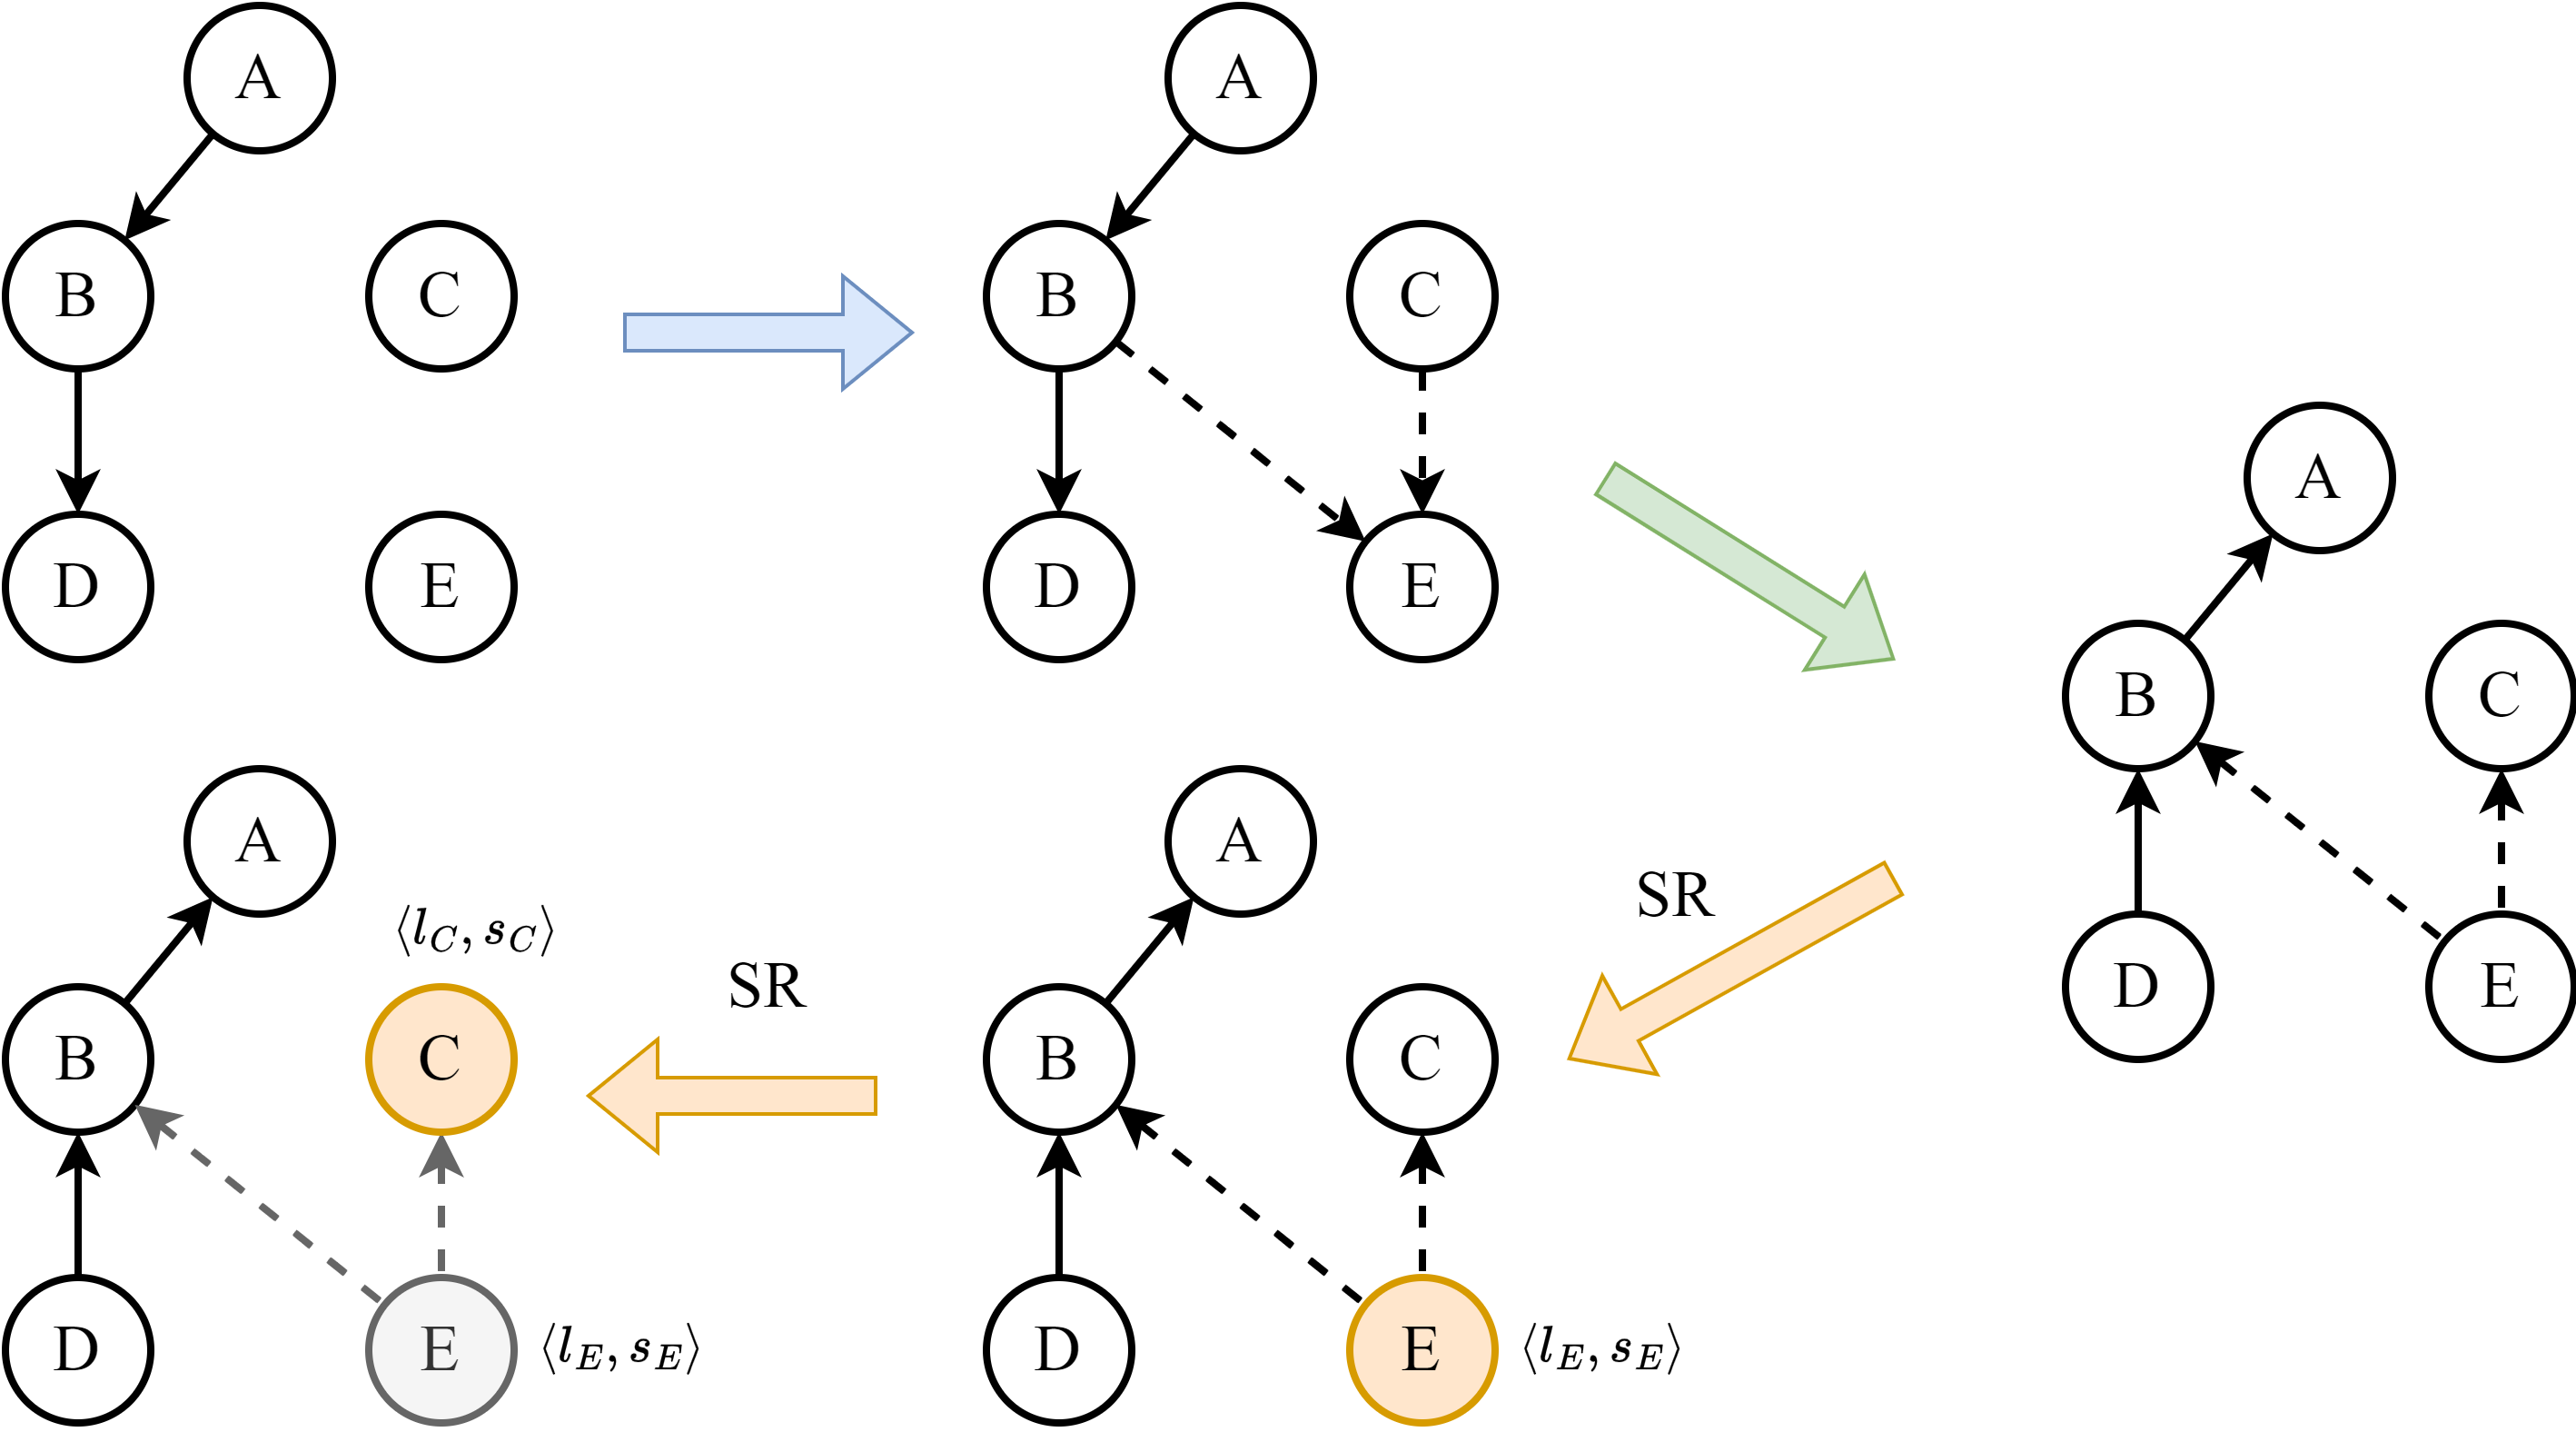
\includegraphics[width=0.8\textwidth]{img/cg_transition.drawio.png} % 调整图片宽度为文本宽度的50%
    \caption{Construction and transformation of $\mathcal{ACG}$} % 添加图片标题
    \label{fig:acg_transform} % 设置图片标签,方便引用
\end{figure}


% 作为HyBinMAS的开端,HSDA接受一个待分析的函数(例如例如libnative-lib.so[+0x1234])及其所在的二进制作为初始输入,进行动静态混合分析。由于HSDA是HyBinMAS框架的基础服务之一,其输出信息是其余环节的重要依据。现有的研究(SymGen)表明,相较于反汇编代码,反编译代码对函数语义理解的贡献度更大,所以我们也将反编译代码作为HSDA模块的一个重要输出供后续使用。在此基础上,HyBinMAS还做了如下突破:

% 我们洞察到这样的伪C代码不能严格代表实际的执行顺序。相反,反汇编代码可以与实际执行的指令具有高度地对齐性。偶一我们在设计HSDA时也将反汇编代码作为另一个输出成分以供后续EV使用。我们还利用HSDA获取了函数的签名信息,包括参数与返回值的类型、存储位置等。这些信息除了为后续SR推理函数名提供基本的支持,还将作为生成与执行测试样例的重要依据。

% 为了解决C2,我们指出在进行语义理解时应当考虑函数调用情况,而且由于C/C++中广泛存在间接调用的使用(例如图xxx),仅考虑静态调用信息将难以保证调用链的完整性,进而影响函数名恢复的效果。所以我们首先定义了带属性的调用图ACG = <AN, AE>,其中节点集AN = N * L * S的每个元素是一个<n, l, s>三元组,分别表示当前节点的标识符、SR预测的函数名和摘要。而边集AE= AE_d + AE_s = N * N * CS * EXP代表了函数之间存在的静态调用和静态调用关系(均由调用者指向被调用者),由<n_u, n_v, cs, exp_{cs}>表示这条边所对应的调用点以及该调用点在反编译代码中对应的调用表达式。

% 其次使用静态分析工具可以获得初始的ACG,它由不携带属性的节点信息和包含属性的静态调用边信息组成,节点的属性信息的补充将会在SR部分详细交待。而对于动态调用边信息,我们首先获得<cs, ct> \in CS * N的调用信息,并定义了公式xxx完成动态增强的过程:
% $AE_d = \{ \langle n_u, ct, cs, exp_{cs} \rangle | \forall n_u \text{ contianing cs}, ct, cs, exp_{cs} \text{ is calling expression aligned with cs} \}$
% 图xxx的蓝色箭头也描述了动态增强的过程,在没有使用动态增强之前,ACG中只有A、B、D之间存在静态调用关系,利用公式xxx,我们在图中用虚线箭头补充了动态调用的关系。


% \begin{algorithm}[htbp]
%   \caption{Dynamic-Enhanced Call Analysis}
%   \label{alg:CallAnalysis}
%   \begin{algorithmic}[1]
%     \REQUIRE $S$: Static call relations, indexed by caller functions
%     \ENSURE $CG$: Dynamic-enhanced Call Graph

%     % \STATE \textbf{// Integrate dynamic call relations into the static set}
%     \FORALL{$\langle cs, ct \rangle \in \texttt{dynamic\_call\_analysis}(binaries)$}
%       \STATE $caller \gets \texttt{get\_function}(cs)$
%       \STATE $S_{caller} \gets S.\texttt{pull}(caller)$
%       \STATE $S_{caller} \gets \texttt{add\_call\_relation}(S_{caller}, \langle cs, ct \rangle)$
%       \STATE $S.\texttt{Push}(S_{caller})$
%     \ENDFOR

%     \STATE $ACR \gets \varnothing$
%     % \STATE \textbf{// Align call targets with decompiled call expressions}
%     \FORALL{$\langle cs, exp_{cs} \rangle \in \texttt{extract\_expressions}(binaries)$}
%       \STATE $cts \gets \texttt{get\_call\_targets}(S_{caller}, cs)$
%       \STATE Add $\langle exp_{cs}, cts \rangle$ to $ACR$
%     \ENDFOR

%     \STATE $CG \gets \texttt{construct\_call\_graph}(ACR)$
%     \RETURN $CG$
%   \end{algorithmic}
% \end{algorithm}

% The first part of Algorithm~\ref{alg:CallAnalysis} (lines 1–6) augments static call relations with dynamically observed calls, producing a more comprehensive set of call relation.
% Since a single call site may correspond to multiple calltargets, $S_{caller}$is implemented as a mapping from a call site to the set of its possible targets, and is updated in Lines 3–5. For the same reason, the second part of the algorithm (Lines 7–11) aligns each callsite’s target set with its corresponding call expression in the decompiled code.Finally, the \texttt{construct\_call\_graph} function generates the dynamic-enhanced call graph based on the aligned relations.
% 算法xxx的第1-6行为静态调用关系补充动态调用,形成一个更加完备的调用关系。由于每个函数的每个调用点可能有多个调用目标,因此$S_{caller}$实际上是一个以调用点为key,以该调用点对应的所有调用目标集合为value的集合,我们使用3-5行更新它。处于相同的原因,我们需要将这样的调用关系在反编译代码中体现,所以算法第7-11将调用点的调用目标集合与反编译代码中对应的调用表达式对齐。最后通过construct_callgraph函数构造一个调用图。






\subsection{Executor Service}
To the best of our knowledge, existing research on binary function name recovery\cite{SymGen, FoC, SymLM, AsmDepictor, XFL} remains confined to the use of static information. Although approaches such as SymLM\cite{SymLM} attempt to incorporate execution behavior, they rely on static call graph data to simulate dynamic behaviors, which still fundamentally belongs to static analysis. To address \textbf{Challenge 3}, we introduce Executor, a novel component designed to emulate the dynamic debugging techniques widely used in manual reverse engineering. In manual analysis workflows, dynamic debugging typically relies on the Debugger functionality provided by tools such as Ghidra\cite{Ghidra} to perform step-by-step execution. While some prior studies have made preliminary attempts in this direction, the gap between their methods and practical usability remains substantial. Moreover, the primary goal of HyBinMAS is not to fully replicate traditional dynamic debugging. Instead, we execute the target function without interruption and capture two specific categories of runtime information:
\begin{enumerate}
    \item function arguments and return values.
    \item trace at the instruction level.
\end{enumerate}

In HyBinMAS, function arguments and return values are tightly coupled with the test case generation process, which will be discussed in detail in the design of the TG. Here, we focus on the instruction set trace information provided by Executor.

When executing a function, a wide range of runtime data can be collected, including context state, call stack information, and the contents of any valid memory address space. Collecting all such data would cause severe context overflow. However, we observe that compilers, when translating source code into assembly (or machine instructions), tend to follow a convention of using registers as much as possible for data storage and computation. Based on this observation, we hypothesize that a function’s register operations can serve as an effective proxy for its memory operations, and therefore select register state information as the primary content of the trace. Since the execution of each instruction alters the context state, providing context at the granularity of instruction is a reasonable choice. However, modern processor architectures typically expose a large number of user-visible registers. Including the full set of register states for every instruction would not only exceed the context window limitations of LLMs but could also incur hallucination risks. To mitigate these issues, we apply the following optimizations:
\begin{itemize}
    \item \textbf{minimize register coverage by excluding trivial registers such as the instruction pointer (IP) while retaining all general-purpose and floating-point registers}; and
    \item \textbf{highlight register state changes by providing the complete register state only at function entry and exit, while for intermediate instructions, including only the registers whose values differ from those in the preceding instruction}
\end{itemize}
%Subsequent experiments confirm that these optimizations help the model focus more effectively on the semantics of each instruction, thereby improving the overall accuracy of semantic understanding.
% 增加一个trace的示例?考虑ARM64 的寄存器种类?


% \subsubsection{Acquiring Trace Information}

% We construct the trace using CPU context information, specifically the state of the registers. This approach is chosen because the ARM64 architecture provides a significantly larger number of programmer-visible registers compared to the x86 architecture. As shown in Table~\ref{tab:arm_registers}, the ARM64 architecture offers 32 general-purpose registers and 32 vector registers. The general-purpose registers can act as units of different sizes (ie. 1B, 2B, 4B and 8B) depending on the operation type. The vector registers are even more versatile, supporting parallel computations in addition to using their lower 32 bits to represent \texttt{float} values and their lower 64 bits for \texttt{double} values. Furthermore, these registers are preferentially used for passing arguments and return values, as well as for storing temporary variables.

% Since the execution of each instruction alters the context state, providing context at an instruction-level granularity is a trivial approach. However, given the large number of registers in the ARM64 architecture, providing the complete register state for every instruction would significantly exceed the context window of an LLM and could also induce hallucinations. Therefore, we implemented the following optimizations:
% \begin{enumerate}
%     \item \textbf{Minimize Register Information:} We select all general-purpose registers. For vector registers, we only consider common access patterns, namely as \texttt{float} and \texttt{double} values.
%     \item \textbf{Differential Tracing:} We provide the complete register state only at the function's entry and exit points. For each intermediate instruction, we only report the registers that have changed relative to the previous step. Subsequent experiments demonstrate that this approach helps the model focus on the semantics of individual instructions, thereby improving the overall accuracy of semantic understanding.
% \end{enumerate}

% \subsubsection{Acquiring Parameters and Return Values}

% Although the standard calling convention in the ARM64 architecture dictates that parameters and return values are passed via registers, which implies that, in most cases, this information would already be captured within the execution trace, we find it beneficial to handle them explicitly. Because parameter and return value information is highly indicative of a function's semantics, highlighting it can significantly aid the LLM in its semantic comprehension. To this end, we leverage Ghidra's static analysis capabilities to precisely identify these values. This process also enables the discovery of parameters stored on the stack.

\subsection{Semantic Restorer Agent}
\label{sec:sr_design}

The \textbf{Semantic Restorer (SR)} constitutes the core component of the \textbf{HyBinMAS} framework. Its primary responsibility is to generate the predicted function name, which serves as the final output of the entire system. To address \textbf{Challange 2} and enhance the effectiveness of name recovery, the \textbf{SR}'s analysis of any given function should incorporate information about its callees. To facilitate the propagation of semantic information between functions, we designed the SR to output not only the inferred name but also corresponding functional summary. The summary is widely recognized in related binary analysis research\cite{SymGen, FoC} as an effective bridge to narrow the knowledge between binary function semantics and the descriptive richness.

In the workflow of traditional binary function name recovery, the aggregation and interpretation of available information have historically been manual endeavors. This manual process is a primary contributor to the tedious and challenging nature of reverse engineering, as it demands significant domain expertise and careful consideration of how to properly leverage both static and dynamic information. Previous research has already demonstrated the non-negligible potential of LLM in both source-level\cite{cs_chatgpt, multi_intent_LLM, statement_cs_LLM, LLM_cs, scs_via_LLM, structured_cs_hyctx, cs_beyond_function, CORE, Calibration_LLM_cs, SimLLM} and binary-level \cite{shang_how_2024, SymGen, FoC, Bin2Summary, BinMetric, DeGPT} understanding tasks. Consequently, we position an LLM as the central component of \textbf{SR}. Nevertheless, a considerable gap persists between the inference of existing methods \cite{SymGen, XFL} and the gold name. Upon careful scrutiny of their approaches, we identified a common shortcoming: they do \textbf{NOT} effectively leverage contextual information, often relying solely on the target function's decompiled code as the basis for inference. Building upon the insights from existing research while addressing their limitations, we have engineered the SR to accept a richer set of inputs:

\begin{enumerate}
    \item \textbf{Static Analysis Artifacts:} As indicated by the black arrow from \textbf{HSDA} to \textbf{SR} in Figure~\ref{fig:overview}, it includes the decompiled code $p$, Attributed Call Graph of target function $\mathcal{ACG}_o$ and $metadata$ about the binary and the function under analysis. This information forms the foundation for semantic understanding, where the inclusion of the call graph is specifically intended to improve the accuracy of inference.
    \item \textbf{Generated Test Cases:} Represented by the dashed orange arrow from \textbf{TG} to \textbf{SR}, it provides the \textbf{SR} with the specific inputs that will be used to probe the function's dynamic behaviors.
    \item \textbf{Execution Feedback:} The red arrow from \textbf{EV} to \textbf{SR} signifies the feedback information consolidated by the \textbf{EV}. This feedback is derived from the execution traces (or errors) produced by the Executor using the \textbf{TG}'s test cases (see Section~\ref{sec:ev_design} for details).
    \item \textbf{Callee Semantics:} The semantic information (i.e., the function name and summary) of the functions called by the target function.
\end{enumerate}

We meticulously orchestrate this multifaceted information into a structured prompt, as depicted in Figure~\ref{fig:prompt_sr}, to serve as the input to the LLM. It is important to note that during its initial inference pass, the \textbf{SR} can only utilize the static information. However, in subsequent iterations, \textbf{HyBinMAS} enriches the context of the \textbf{SR} with dynamic information derived from \textbf{Executor}, \textbf{TG} and \textbf{EV}, enabling LLM to progressively refine its inference.

\begin{figure}[h] % [h] 表示图片放置在当前位置
    \centering
    \includegraphics[width=0.8\textwidth]{img/prompt_sr.drawio.png} % 调整图片宽度为文本宽度的50%
    \caption{Construction and transformation of $\mathcal{ACG}$} % 添加图片标题
    \label{fig:prompt_sr} % 设置图片标签,方便引用
\end{figure}


Building upon the $\mathcal{ACG}$ obtained from \textbf{HSDA}, we abstract the core operation of \textbf{SR} as a state transition function. This function describes how applying the \textbf{SR} to a specific node \(n\) in the current graph \(\mathcal{ACG}\) results in a new graph state, \(\mathcal{ACG}'\):
\begin{equation}
\label{eq:sr_transition}
\mathcal{ACG}' = \text{SR}(n, \mathcal{ACG})
\end{equation}

The effect of this transformation is to produce an updated graph, \(\mathcal{ACG}'\), where the attributes of the vertex \(n\) have been newly populated. The difference between the graphs can be expressed as the augmentation of \(n\) with a predicted name \(l\) and summary \(s\). This process, where the SR enriches a node with semantic information, is visually depicted by the blue arrows in Figure~\ref{fig:acg_transform}.

% A critical prerequisite for applying this transition function is to process the graph's nodes in a bottom-up, reverse topological order. To facilitate this, we first operate on the **transpose** of the ACG. This operation, as illustrated by the green arrows in Figure~\ref{fig:xxx}, involves reversing the direction of every edge in the graph. The resulting structure, denoted as \(\mathcal{G}^T\), ensures that when we traverse the nodes, a function's callees are typically analyzed before the function itself, allowing semantic information to propagate upwards through the call hierarchy.

We also designed the workflow shown in Algorithm \ref{alg:sr_workflow} for \textbf{SR}, where the input $o$ denotes the objective function, $\mathcal{ACG}_o$ is the output of \textbf{HSDA}, which consists of all nodes and edges reachable from $o$, $cases$ represent the test cases generated by \textbf{TG}, and $feedback$ refers to the feedback information from \textbf{EV}. The algorithm outputs the predicted name of the objective function.

\textbf{Line~1} of the algorithm uses \texttt{get\_sub\_ACG} to obtain the subgraph ${\mathcal{ACG}_o}$, . Without considering recursion, the call graph is essentially a \textbf{Directed Acyclic Graph (DAG)}, from which we can obtain its \textbf{reverse topological order}. For recursive calls, there must exist a \textbf{back edge}, which can be removed to obtain a DAG as well. The \texttt{reverse\_topo\_sort} operation in \textbf{line~2 of Algorithm \ref{alg:sr_workflow}} is responsible for this task. Lines~8--12 of the algorithm describe the process of \textbf{enhancing LLM inference with both call information and dynamic information}.



\begin{algorithm}
  \caption{Workflow Algorithm for SR}
  \label{alg:sr_workflow}
  \begin{algorithmic}[1]
    \REQUIRE $o$: The offset of target function, $\mathcal{ACG}_o$: The Attributed Call Graph from HSDA, $cases$ The test cases from TG, $feedback$: The feedback from EV
    \ENSURE $l$: The predicted function name

    % \STATE {$\mathcal{ACG}_o) \gets \texttt{get\_sub\_ACG}(\mathcal{ACG}, o)$}
    \STATE {$W \gets \texttt{reverse\_topo\_sort}(\mathcal{ACG}_o)$}

    \STATE {$LC \gets \varnothing$}
    \FORALL{$n_u \in W $}
        \IF{$n_u \in LC$}
            \STATE {$\langle l, s \rangle \gets \texttt{get}(LC, w)$}
        \ELSE
            \STATE {$fact_{callees} \gets \cup_{\langle n_u, n_v, cs, exp_{cs} \rangle \in \mathcal{E}(\mathcal{ACG}_o) \land \langle n_v, l_v, s_v \rangle \in \mathcal{N}(\mathcal{ACG}_o) }{\langle l_v, s_v \rangle} $}
            \STATE {$\langle l, s \rangle \gets \texttt{query\_LLM}(n_u, fact_{callees})$}
            \IF{$feedback \ne NULL$}
                \STATE {$\langle l, s \rangle \gets  \texttt{query\_LLM}(n_u, fact_{callees}, cases, feedback)$}
            \ENDIF
            \STATE {$\texttt{set}(LC, n_u, \langle l, s \rangle)$}
        \ENDIF
    \ENDFOR
    \RETURN $l$
  \end{algorithmic}
\end{algorithm}


% SR是HyBinMAS的核心组件,它的主要输出信息之一是预测出的函数名,这同样也是HyBinMAS的最终输出。考虑到C2的存在,为了提升函数名恢复的效果,SR在分析一个函数时还需要考虑它所调用的函数。为了能够在不同函数之间传递语义信息,我们在设计SR时除了用于预测函数名之外,还需要输出函数的摘要信息,这在许多二进制逆向相关的研究中都被认为是表征函数语义的有效方式。

% 在传统二进制函数名恢复任务的流程中,如何将现有的信息汇总起来并将进行推理一直都由人工负责,这也是二进制逆向任务繁琐困难的原因之一,因为它同样需要一定的领域知识,而且需要考虑如何妥善地利用这些静态信息与动态信息。先前的研究已经展现了LLM在源码级任务、二进制级任务中具有不可忽视的潜力,因此我们在提出HyBinMAS时就将LLM作为核心组件,SR就是其中之一。但是现有的研究的成果(SymGen、XFL)与理想结果仍然存在较大的鸿沟,我们仔细学习与审视了他们的方法,发现它们并没有很好地利用上下文信息,而通常仅仅将目标函数的反编译代码作为推断的依据。在借鉴了现有研究的经验、总结了他们的不足的基础上,我们为SR设计了如下的输入信息:

% 1. 图xxx中由HSDA到SR的黑色箭头表示了反编译代码、调用图、关于待分析文件和函数的元信息等。这些信息是语义理解的基础,我们通过引入调用图来增加函数语义理解的准确度。
% 2. 从TG到SR的橙色虚线箭头代表了生成的测试样例
% 3. 从EV到SR的红色箭头则是EV根据TG的测试样例和Executor的执行信息总结得到的反馈信息(具体见xxx)
% 4. 目标函数所调用的函数的语义信息(函数名和摘要)

% 我们将这些信息按照图xxx所示的方式妥善编排成提示词作为LLM的输入。值得注意的是,SR在首次推测函数名时,它能够利用的信息只有(1)中的静态信息。但在后续的迭代中,HyBinMAS就可以根据Executor、TG和EV的输出,为SR提供必要的动态信息以改进LLM的推测结果。


% 我们在HSDA获得的ACG的基础上,将SR抽象为公式xxx所示的状态转移方程,它表示对于当前状态的ACG,且指针位于节点n处,经过SR之后ACG的状态变为ACG^\prime,其中ACG^\prime - ACG = <n, l, s>,也即SR对节点n所代表的函数名和摘要信息进行了补充。图xxx的橙色箭头形象地描述了这一过程
% $$ACG^\prime = SR(n,ACG)$$


% 我们还为SR设计了算法xxx所示的工作流,其中输入ACG是HSDA的输出结果,o代表目标函数,cases代表由TG产生的测试案例,feedback则是EV的反馈信息,该算法输出目标函数的预测名称。算法的第1行利用get_sub_ACG获得了从目标函数o能遍历到的所有节点和边组成的子图ACG_o。在不考虑递归的情况下,调用图实际上是一个有向无环图,我们可以获得它的反向拓扑序列;而对于递归调用,它必然存在一条回边,我们可以将这样的回边删除,仍然可以得到一个有向无环图,算法xxx中的第2行的topo_sort正是负责这一任务。而算法8-12行则描述了调用信息和动态信息增强LLM推理的过程。




\subsection{Test Generator Agent}
\label{sec:tg_design}

We reiterate that semantic understanding based solely on static information is often insufficient and imprecise. To emulate the process of manual dynamic debugging, it is necessary not only to provide execution support via the Executor but also to construct appropriate test cases. Within \textbf{HyBinMAS}, this functionality is realized by the \textbf{Test Generator (TG)}. However, test case generation is a non-trivial task, particularly because \textbf{HyBinMAS} requires test cases that can intelligently validate the function's anticipated logic. Consequently, we employ a LLM as the core of the \textbf{TG}. Furthermore, the design of the \textbf{TG} should navigate these significant obstacles:

\begin{enumerate}
    \item \textbf{Unlike conventional test case generation tasks\textbf{[TODO]}, the TG must infer potential parameters and their corresponding types---including primitive types, their derivatives (e.g., pointers), and custom structures---directly from decompiled code, without access to the original source. This significantly complicates the generation process.}
    \item \textbf{The generated test cases must be concretely applicable to the target function, meaning they must be translated into actually executable code.}
    \item \textbf{Accurately recovering the full parameter and return value information from stripped binaries is, in the general case, an undecidable problem.\cite{sig_meet_opt}}
\end{enumerate}

To manage these complexities, we decompose the \textbf{TG} into two core components as depicted in Figure~\ref{fig:overview}: the \textbf{Orchestrator} and the \textbf{Materializer}, responsible for the high-level design and the concrete implementation of the test cases, respectively.

First, the \textbf{Orchestrator} is tasked with designing the test cases.  It receives the target function's semantic information and generates a test plan articulated in natural language, aimed at verifying the logic implied by the SR's semantic description, namely the function summary. The rationale for this separation is twofold: different architectures and instrumentation tools often demand distinct implementation strategies and, thus, different domain knowledge; Entrusting both the design and implementation to a single LLM would dramatically increase the risk of context overflow. To facilitate implementation by the Materializer, the Orchestrator's design must explicitly specify the input values for parameters, the expected output values for both parameters and the function's return value. Figure~\ref{fig:example_orchestrator_output}. In conclusion, our Orchestrator first uses an LLM for test case generation. To validate  correctness of pointer operations, we then leverage program slicing \textbf{[TODO]} to extract parameter-related statements from the decompiled code, which a secondary LLM reviews to ensure the integrity of these critical operations within the proposed test plan.

\begin{figure}[h] % [h] 表示图片放置在当前位置
    \centering
    \includegraphics[width=0.8\textwidth]{img/example_orchestrator_output.drawio.png} % 调整图片宽度为文本宽度的50%
    \caption{Construction and transformation of $\mathcal{ACG}$} % 添加图片标题
    \label{fig:example_orchestrator_output} % 设置图片标签,方便引用
\end{figure}

Second, the \textbf{Materializer} component translates the natural language descriptions from the Orchestrator into executable code using specific memory manipulation primitives; this process is effectively a code generation task. To address obstacles (1) and (2), we must furnish the LLM with sufficient domain-specific knowledge\textbf{[TODO]}. In our reference implementation, for example, we provide the LLM with the relevant memory manipulation APIs from the Frida toolkit (see Appendix for details). Moreover, instead of presupposing the form of the function's arguments, we prompt the LLM to generate a dedicated function (e.g., \texttt{writeArgs}) to marshal the parameters according to the test case's input requirements. For the same reason, the LLM is also instructed to generate a corresponding \texttt{readArgs}-like function to read the output parameters and return them as a string containing explanatory details. The return value is handled similarly. Figure~\ref{fig:example_materializer_output} illustrates the materialized implementation corresponding to the design from Figure~\ref{fig:example_orchestrator_output}.

\begin{figure}[h] % [h] 表示图片放置在当前位置
    \centering
    \includegraphics[width=0.8\textwidth]{img/example_materializer_output.drawio.png} % 调整图片宽度为文本宽度的50%
    \caption{Construction and transformation of $\mathcal{ACG}$} % 添加图片标题
    \label{fig:example_materializer_output} % 设置图片标签,方便引用
\end{figure}

Finally, acknowledging the difficulty posed by obstacle (3), we anticipate that a test case initially generated may fail to execute. We therefore establish an iterative improvement between the Executor and the \textbf{TG}: When the Executor fails to run a materialized test case, it reports back essential information via error messages or exceptions, which is then used to refine the implementation in the Materializer. Successfully executed test cases, along with their execution traces, are passed to the \textbf{EV} for analysis. For the same reason, we have incorporated a dynamic execution fallback strategy: if the Materializer's implementation attempts fail more times than the specified threshold $R$, \textbf{HyBinMAS} will abort the execution of that particular test case and pass the error information directly to the \textbf{EV} for analysis.

% 我们再次强调,仅仅根据静态信息来进行语义理解时不准确的,为了模拟人工动态调试的过程,我们除了在Executor部分提供相关的运行支持之外,还需要为其构造合适的测试样例并“触发”目标函数的执行。在HyBinMAS中,我们设计了TG来实现这样的功能。然而,测试样例生成同样不是一个trivial的任务,尤其是HyBinMAS还要求测试样例需要智能地验证目标函数的预期逻辑。所以我们使用LLM作为TG的核心。然而,设计TG时,需要解决如下关键问题:(1)不同于一般的测试样例生成任务,TG需要在不知道源码的情况下分析反编译代码中可能用到的参数及其对应的类型,包括基本类型及其衍生类型、自定义类型或其他更复杂的情况,这无疑增加了测试样例生成的困难性。(2)生成的测试样例必须能够被正确地应用到目标函数上,也就是说它是一段实际可执行的代码。(3)准确恢复stripped binaries中的函数参数与返回值信息是一个不可判定任务。所以我们将TG拆分为图xxx所示的两个核心组件:Orchestrator和Materializer,分别负责测试样例的设计编排与实现

% 首先,我们使用Orchestrator完成测试样例的设计任务,它接收目标函数的语义信息测试目标,生成一种由自然语言编写的测试样例i验证该语义信息所体现的逻辑。这样设计的合理性在于:对于不同的架构和不同工具,我们通常需要不同的实现方式(例如编写不同的测试代码),这意味着不同的领域知识。如果直接将测试样例的设计与实现都交给同一个LLM完成,将极大增加上下文溢出的风险。为了便于Materializer实现测试样例,我们需要在设计时明确地输出参数的输入值、参数与返回值的预期值。所以我们按照了图xxx所示的格式作为Orchestrator的输出。请注意,要想正确地获取这些信息并不是轻而易举的事,尤其是当参数是指针类型时,所以我们在实现Orchestrator时,除了使用一个LLM生成测试样例,我们还利用程序切片技术将反编译代码中与参数相关的语句提取出来,并利用另一个LLM对其中涉及的指针操作进行review,确保测试样例中指针操作的正确性。

% 其次,Materializer组件会根据Orchestrator的自然语言描述,使用特定的内存操作代码实现出来,所以这实际上是一个函数生成任务。为了应对问题(1)与问题(2),我们需要给LLM足够多的领域知识。以本文的实现为例,我们需要提供Frida中内存操作的相关API(详细件附录)。而且我们不能提前假设参数的形式,而是应当提示LLM生成一个函数(例如writeArgs)来修改参数使其满足测试样例的输入要求。另外,处于同样的原因,我们也需要让LLM生成一个形如readArgs的函数来读取参数并以一个包含解释信息的字符串的形式返回(返回值也有相同的要求)。图xxx展示了图xxx所对应的实现结果。

% 最后,我们承认问题(3)的困难性,单次生成的测试样例很有可能在Executor上执行不起来,所以我们增加了Executor和TG之间的交互:当Executor无法执行TG实现的测试样例时,它会以报错或异常的形式反馈必要的信息并用于Materializer的改进。最终通过的测试样例会与Executor执行成功的信息一同交给EV分析。处于同样的原因,我们还涉及了动态执行的fallback策略:当Materializer实现失败次数超过了指定阈值时,HyBinMAS会放弃执行该测试样例,并直接将错误信息和对应的测试样例交给EV进行分析。


\subsection{Execution Validator Agent}
\label{sec:ev_design}

In HyBinMAS, dynamic information is incorporated to address \textbf{Challange 3}. This dynamic information includes the execution information from the Executor and the test cases generated by TG. However, such data can be excessively verbose and may contain irrelevant noise. Directly feeding this information into SR would lead to context overflow and hallucination issues. To mitigate these risks, HyBinMAS employs the \textbf{Execution Validator (EV)} to analyze and condense the information into concise, well-structured natural language descriptions before feeding it back to the \textbf{SR}.

As depicted in the red rectangular of Figure~\ref{fig:overview}. For each test case, if execution fails, the Fallback Analyzer interprets and summarizes the cause of failure. Otherwise, the Normal Analyzer examines the Executor’s execution results and, based on the test cases provided by the TG, determines whether the observed results match the expected outputs. If they do, the case is simply marked as passed; otherwise, the actual execution results are summarized and converted into feedback information. The results for all test cases are then aggregated and fed back to the SR for the next iteration, continuing until all test cases pass verification or the iteration limit is reached.

Evidently, the Fallback Analyzer and Normal Analyzer constitute the core components of the \textbf{EV}. For the Normal Analyzer, we construct a prompt template by combining the \textbf{SR}’s semantic understanding, the \textbf{TG}’s test cases, and the Executor’s execution information, as illustrated in Figure~\ref{fig:prompt_ev_nm}, and pass it to the LLM. For the Fallback Analyzer, we organize the failed test cases and their corresponding error messages into a query format, as shown in Figure~\ref{fig:prompt_ev_fb}, before submitting it to the LLM.

% 我们在HyBinMAS中添加动态信息的目的是为了解决C3。这些动态信息包括Executor的执行信息、错误信息和TG生成的测试样例。然而它们可能十分冗长,而且可能包含其他干扰信息,如果直接将这些信息输入给SR,同样也会招致模型上下文溢出和幻觉的问题,所以HyBinMAS使用EV将这些信息进行分析并总结成合适的自然语言描述,再反馈给SR。
% 对于每一个测试样例,如果执行失败,则由Fallback Analyzer解读并总结失败原因,否则由Normal Analyzer分析Executor的执行结果,并根据TG提交过来的测试样例,判断该测试样例的执行结果是否符合预期结果,如果预期则简单标记为通过,否则需要总结实际的执行结果并形成反馈信息。所有样例的结果会被汇总并反馈给SR进行下一轮迭代,直到所有的测试样例都验证通过,或者迭代次数耗尽。
% 显然,Fallback Analyzer和Normal Analyzer是EV的核心。对于Normal Analyzer,我们将SR的语义理解结果、TG提交的测试样例和Executor的执行信息按照图xxx所示的方式组成提示词模板并交给LLM。对于Fallback Analyzer,我们将执行错误的测试样例和对应的错误信息按照图xxx所示的方式组织成查询并提交给LLM



\section{Implementation and setup}


\subsection{Dataset Construction}

To objectively evaluate the applicability of our tool across multiple architectures and to facilitate direct comparison with existing baseline methods, our benchmark is divided into two distinct parts. The first part, Baseline Benchmark\cite{SymGen}, comprises datasets that are widely adopted by prior works, covering architectures such as x86-64, x86-32, ARM-32, and MIPS. The second part, ARM-64 Benchmark, is a newly curated dataset specifically targeting the ARM-64 architecture. This dataset is manually collected and constructed from various open-source repositories, addressing the lack of publicly available ARM-64 datasets in the existing literature.

\begin{figure}[t] % [h] 表示图片放置在当前位置
    \centering
    \includegraphics[width=0.5\textwidth]{image/ConstructDataset.drawio.png} % 调整图片宽度为文本宽度的50%
    \caption{An overview of the dataset construction process} % 添加图片标题
    \label{fig:construct-dataset} % 设置图片标签,方便引用
\end{figure}


\renewcommand\arraystretch{1.31}
\begin{table}[tb]
  \centering
  \footnotesize
  \caption{Data set statistics for Benchmarks}\label{table:data}
    \begin{tabular}{p{2.5cm}p{1.6cm}p{1.6cm}p{1.6cm}p{1.6cm}p{1.6cm}p{1.6cm}}
   \toprule
     & Architecture & Optimization & \#Variables & \#Instructions &\#Functions\\
    \hline
    Baseline Bench  & 8 & 30\\
    - x86-64 &1,195,994 & 7,634,717\\
    - x86-32 &1,195,994 & 7,634,717\\
    - MIPS &1,195,994 & 7,634,717\\
    - ARM-32 &1,195,994 & 7,634,717\\
    ARM-64 Bench  &1,195,994 & 7,634,717\\
    \bottomrule
  \end{tabular}
  \vspace{-0.2in}
\end{table}
\renewcommand\arraystretch{1.0}


\subsubsection{Baseline benchmark}
Many studies in function name recovery utilize projects from the GNU ecosystem to construct dataset. For instance, SymGen\cite{SymGen} manually compiled 33 GNU projects to construct their evaluation dataset. To ensure a fair and direct comparison with our baselines, we replicated the dataset construction methodology proposed by SymGen. It is important to note that the original SymGen dataset is extensive, comprising a vast number of functions from both executable files and shared libraries. Constrained by the token consumption of the \textbf{HyBinMAS} framework, and to establish a level playing field with the dataset we introduce later, we elected to extract only the shared library files from their collection for RQ1. Furthermore, the original dataset provided by SymGen contains only decompiled code and lacks other artifacts required by \textbf{HyBinMAS} (such as assembly code and call graphs). We therefore processed the binaries to supplement this dataset with the necessary additional information. %The statistical details of the resulting dataset are presented in Figure~\ref{fig:symgen_dataset_stats}.



\subsubsection{ARM-64 benchmark}
To the best of our knowledge, no dedicated dataset currently exists for semantic understanding tasks on Android Native Libraries, such as function name recovery and comment generation. Although numerous data sets are available for stripped binaries, they are inadequate for our purposes. These existing datasets either lack compilation variants for the ARM64 architecture or are not executable on Android devices, which is unacceptable for our method. Therefore, we are working on the construction of a new specialized dataset. The overview of this process is illustrated in Figure~\ref{fig:construct-dataset}.

\textbf{1)Android Project Selection}. Our ultimate objective is to analyze closed-source applications. Therefore, the primary principle guiding our selection of open-source projects is to ensure they accurately reflect the characteristics of their closed-source counterparts. Inspired by BinMetric\cite{BinMetric} and BinaryLLM-Eval\cite{BinaryLLM-Eval}, we adapt and extend their critera to align with the specific requirements of our work:

\begin{itemize}
    \item \textbf{Executability:} The requirement for executability is twofold. The first consideration is practical applicability, necessitating that the target application be runnable. The second is the operational constraints imposed by the Executor within our proposed approach.

    \item \textbf{Native Code  Availability:} Selected projects must contain native source code (implemented in C or C++). This is crucial as projects providing only pre-compiled .so files would prevent us from obtaining the ground-truth function semantics (i.e., names and comments). It is critical that the target functions must be non-exported. This ensures that their symbol information can be completely removed during the stripping process without impairing the application's runtime functionality—a task that is infeasible for exported functions.

    \item \textbf{Realisticity and Modernity:} To ensure the dataset reflects contemporary and real-world scenarios, the selected projects must be compatible with the recent Android versions. At the time of our data collection, with Android 14+ gradually becoming the mainstream system, we established Android 15 compatibility as our target standard.

    \item \textbf{Project Quality:} High-quality projects are essential, as factors like code clarity and structure can significantly influence the performance of semantic analysis. We identified quality through characteristics such as a well-organized project structure, clear logical implementation, and adherence to good naming conventions. Project quality can be quantifiedby its Stars and Forks on GitHub.

    \item \textbf{Domain Diversity:} To comprehensively evaluate the generalization capabilities of our proposed method, the dataset should encompass applications from a broad range of domains. We identify and include projects from the following categories: Communication \& Social Networking,  Science \& Education, Multimedia, Game, Finance and Tools. It is important to acknowledge that these categories do not cover the full spectrum of real-world applications. Numerous projects from other domains were filtered out as their failure to meet the 1st criterion.

    \item \textbf{Maintenance Status:} To ensure the relevance of the compiled binaries and their underlying code, projects were required to have a recent history of updates or maintenance. We have chosen 5 years as the threshold.
\end{itemize}

From an initial survey of \textbf{106} Android application projects, we downloaded \textbf{26} candidates based on the requirements outlined above. During the subsequent compilation and build process, we filtered out any project that could not be constructed as specified (see details below), resulting in a final corpus of \textbf{6} APKs. These artifacts are then subjected to the subsequent processing stages (Steps \normalsize{\textcircled{\scriptsize{3}}}\normalsize–\normalsize{\textcircled{\scriptsize{7}}}\normalsize) illustrated in Figure~\ref{fig:construct-dataset}.


\textbf{2)APK Construction}. We utilized Gradle\cite{Gradle} and \cite{CMake} to complete the build tasks. For each application, we compiled two distinct variants: \textbf{Release} and \textbf{Release-DWARF}. It is important to note that we deliberately avoided the common practice of building a standard Debug version with DWARF information for its Release counterpart. This is because build tools like Gradle and the NDK\cite{NDK} apply different configurations (e.g., varying optimization levels) to Debug and Release builds. Such discrepancies will result in non-identical native code, thereby complicating the subsequent alignment process.

Instead, our approach uses the standard Release as the baseline. We generate the \textbf{Release-DWARF} variant by augmenting the Release binaries with DWARF information while ensuring the underlying machine code remained unchanged. The final executable deployed on the Android system is also the standard Release, which perfectly aligns with real-world scenarios. Consistent with established practices in previous research, we apply Step \normalsize{\textcircled{\scriptsize{3}}}\normalsize and  \normalsize{\textcircled{\scriptsize{4}}}\normalsize to generate the corresponding disassembly, decompiled code, and $\mathcal{ACG}$ for these binaries.


\textbf{3)Ground-Truth Construction}. This process begins with the extraction of native source code from the selected projects (as shown in step \normalsize{\textcircled{\scriptsize{5}}}\normalsize). We designated the developer-written function names as the ground-truth. This was accomplished by parsing the C/C++ source code using tree-sitter\cite{tree_sitter} (\normalsize{\textcircled{\scriptsize{6}}}\normalsize).

\textbf{4)Alignment}. In step \circlenum{2}, we obtained the binary variant that includes DWARF information. This variant shares identical function address offsets with its stripped counterpart, which allows for a straightforward alignment of the function body with their corresponding function name. Furthermore, the DWARF data contains precise records of the source code locations (i.e., file and line number) for each function and variable. This information serves as the definitive basis for aligning the decompiled code with the original source code. Through this two-step alignment process, we can reliably link each function in the binary (represented by both its assembly and deompiled code) to its corresponding ground-truth.


\textbf{5)Filtering and Leakage Check}. To accurately simulate the senarios of real-world applications, we implemented three filtering steps. First, we filtered out any functions that retained their symbol information post-stripping to avoid overestimating the method's performance. Second, we discarded functions with very small bodies (defined as having fewer than 5 assembly instructions). Third, we remove identical functions within a APK according to its Debug info.

Ultimately, we get 6 Android projects and 3996 binary functions for our dataset. Detailed information for each project is presented in Table~\ref{tab:arm_dataset_stats}.
\renewcommand\arraystretch{1.31}
\vspace{-0.5em} % 表格后减少0.5em的空白
\begin{table}[!ht]
    \caption{Statistics of ARM-64 Dataset}
    \label{tab:arm_dataset_stats}
    \centering
    \begin{tabular}{ccccccccccc}
        \toprule
        \textbf{Project} & \textbf{sgtpuzzles} & \textbf{RTranslator} & \textbf{ProtonVPN} & \textbf{FFmpeg} & \textbf{chatAir} & \textbf{BlackDex} \\
        \midrule
        Binaries & 2 & 2 & 4 & 1 & 1 & 2 \\
        Functions & 390 & 25 & 1284 & 152 & 2097 & 18 \\
        \bottomrule
    \end{tabular}
\end{table}
\vspace{-1em} % 表格后减少0.5em的空白
\renewcommand\arraystretch{1.0}


\subsection{Baselines}
Within the domain of function name recovery, we select SymGen\cite{SymGen} as our primary baseline, as it represents the current state-of-the-art (SOTA). We acknowledge that FoC\cite{FoC} is another recent SOTA method; however, its focus is exclusively on cryptographic functions, placing it outside the scope of our general-purpose evaluation. Additionally, considering the formidable capabilities demonstrated by general-purpose LLMs across a wide range of tasks, we also include Deepseek-R1\cite{Deepseek-R1} as a baseline. Prior to SymGen\cite{SymGen}, research in this area predominantly framed function name recovery as a classification task. Therefore, we have selected XFL\cite{XFL} from this line of traditional research to serve as a representative method in our set of baselines.

% \textbf{XFL.}

% \textbf{SymGen.}


\subsection{Evaluation Metrics}
Consistent with prior works\cite{NFRE, NERO, SimLLM, SymGen}, we choose to use metrics based on precision, recall, and F1-score to evaluate the effectiveness of different methods. For a given predicted function name $S_l = \{w_1, w_2, ..., w_m\}$ and its corresponding gold one $\hat{S}_l = \{\hat{w}_1, \hat{w}_2, ..., \hat{w}_n\}$. we first compute TP, FP, and FN through set operations, and then calculate precision, recall, and F1-score based on these values:
% 和之前的工作一致,我们选择使用基于准确率、召回率和F1分数的指标衡量不同方法的有效性。对于给定的参考函数名\hat{S}_l = {\hat{w}_1, \hat{w}_2, ..., \hat{w}_n}和方法预测的函数名S_l = {w_1, w_2, ..., w_m},我们首先通过集合运算计算出TP、FP和FN,之后在此基础上计算出准确率、召回率和F1分数:
$$
TP = |\hat{S}_l \cap S_l|, \ FP = |\hat{S}_l \setminus S_l|, \ FN = |S_l| - TP
$$
$$
\text{Precision} = \frac{TP}{TP + FP}, \text{Recall} = \frac{TP}{TP + FN}, F_{1} = \frac{2 \times \text{Precision} \times \text{Recall}}{\text{Precision} + \text{Recall}}
$$
% 同SymGen和SymLM一样,我们使用CodeWordNet来处理语义相似的单词。
Similar to SymGen\cite{SymGen} and SymLM\cite{SymLM}, we use CodeWordNet to handle semantically similar words.


\subsection{Experimental Setup}
Our implementation leverages \textbf{Ghidra v11.3.2} to procure static information, including disassembly, decompiled pseudo-code, the static call graph, and function signatures. For the acquisition of dynamic call information, we employ \textbf{Simpleperf}. Specifically, we sample execution at a frequency of 1000\,Hz and, to ensure uniform processing, record only the offsets of call sites rather than their symbolic names. The raw output from Simpleperf is a call stack, which we process by identifying contiguous sequences of frames belonging to the same binary module to derive \((cs, ct)\) pairs. We emphasize that while dynamic instrumentation tools like Frida could achieve the same outcome, our empirical evaluation revealed that Frida's instrumentation overhead introduced prohibitive application startup latencies, often causing the target process to hang or be terminated by the operating system.

The implementation of Executor is centered on \texttt{Frida}. We utilize its \texttt{Stalker} engine to trace instruction sequences and thereby capture execution information. Frida's hooking capabilities are instrumental for intercepting the target function, while its comprehensive API provides the necessary primitives for reading and writing register and memory state, as required by TG. A critical design choice is our use of an indirect triggering mechanism. Rather than invoking the target function directly---a precarious approach given that parameters can be exceedingly complex and involve pointer values that are impossible to synthesize correctly, leading to inevitable crashes---we instead hook the function and intercept it during a live execution. This strategy ensures that when our analysis begins, the function's parameters have already been populated with valid values by the program's natural control flow.

Our experiments were performed on a server running Ubuntu 20.04, equipped with a 64-core AMD EPYC 7543 processor at 2.8 GHz, 755 GB memory, and two NVIDIA A100 GPUs with 40 GB VRAM each. All applications in the dataset are deployed on ARM-architecture smartphones equipped with the Android 15 operating system. For the control parameters used in Algorithm~\ref{alg:HyBinMAS}, we set the maximum iterations $M$ to 3, the maximum retries $R$ to 3, and the maximum number of test cases $K$ to 3.


\section{Evaluation}
To evaluate xx, we propose the following research questions.
\begin{itemize}
    \item \textbf{RQ1:} How effective and generalizable is xx compared with the state-of-the-art approaches across different architectures (e.g., x86-64, x86-32, ARM-32, MIPS, ARM64)?
    %在现有benchmark 跑xx静态分析和baseline;在arm64跑xx静态分析+baseline(按原论文逻辑切分测试集数据集?)
    \item \textbf{RQ2:} To what extent does the integration of dynamic analysis and runtime information enhance the accuracy and robustness of function name recovery, particularly in handling complex program behaviors and out-of-vocabulary (OOV) symbols?
    %在arm64数据集跑动态分析,xx动态跑的准确度结果,与xx静态恢复结果相比较,除了准确度提升外,重点分解统计多分析出来的case里 有多少复杂行为(分别是哪些),有多少针对复现的symgen而言的oov数据。
    \item \textbf{RQ3:} How efficient is xx compared with the state-of-the-art approaches? %时间;可按静态xx-1、动态xx-2,将xx且为两个工具来与baseline对比;既显得xx-1快,又能表现出动态xx-2的在时间上的代价
    \item \textbf{RQ4:} How do the individual components of xx contribute to its overall capability for function name recovery? %消融实验
\end{itemize}


\subsection{RQ1: Effectiveness of xx}

\begin{table}[t]
  \centering
  \footnotesize
  \caption{Results of Effectiveness Evaluation}
  \renewcommand\arraystretch{1.15}
    % \begin{tabular}{c|ccccccc|c}
    \begin{tabular}{p{2cm}p{.4cm}p{.4cm}p{.6cm}p{.4cm}p{.4cm}p{.6cm}p{.4cm} p{.4cm}p{.6cm}p{.3cm} p{.3cm}p{.3cm}}
    \toprule
    \multirow{2}*{Projects}& \multicolumn{3}{c}{\textbf{XFL}}&\multicolumn{3}{c}{\textbf{SymGen}}&\multicolumn{3}{c}{\textbf{xx-static}}&\multicolumn{3}{c}{\textbf{xx-dynamic}} \\
    \cline{2-4}\cline{5-7}\cline{8-10}\cline{11-13}
     &  P & R & F1&  P & R & F1&  P & R & F1 &  P & R & F1 \\
    \hline
    Baseline x86-64  \\ 
    - o0 & 0.922 & 0.867 & 0.893 & 0.651 & 0.531 & 0.585 & 0.650 & 0.600 & 0.624 &- &- &- \\
    - o1 \\
    - o2 \\
    - o3 \\
    \hline
    Baseline x86-32 & 0.922 & 0.867 & 0.893 & 0.651 & 0.531 & 0.585 & 0.650 & 0.600 & 0.624 &- &- &- \\
    Baseline MIPS & 0.922 & 0.867 & 0.893 & 0.651 & 0.531 & 0.585 & 0.650 & 0.600 & 0.624 &- &- &- \\
    Baseline ARM-32 & 0.922 & 0.867 & 0.893 & 0.651 & 0.531 & 0.585 & 0.650 & 0.600 & 0.624 &- &- &- \\
    ARM-64 Bench & 0.633 & 0.501 & 0.559 & 0.659 & 0.560 & 0.605 & 0.643 & 0.585 & 0.613 \\
     \hline
    \end{tabular}%
\end{table}%
\renewcommand\arraystretch{1.0}

To evaluate xxx .... we

\subsection{RQ2: Improvement of dynamic analysis}


\begin{table}[t]
  \centering
  \footnotesize
\caption{Recovery results for complex patterns}\label{tab:dy3}
  \renewcommand\arraystretch{1.15}
\begin{tabular}{p{1.7cm}p{1.7cm}p{1.2cm}p{1.2cm}p{1.2cm}p{1.2cm}p{1.2cm}}
\toprule
patterns & sub-pattern &xx dynaic &xx static & xfl &symGen    \\
\midrule
\textbf{Method(19)} & Missing(12) &5 &1 &\textbf{9} &5 &2 \\
\textbf{Method(19)} & Noncallable(6) &5 &1 &\textbf{9} &5 &2 \\
\textbf{Return value(29)} & Noncallable(6) &\textbf{17}&\textbf{5}&0&0&7\\
\bottomrule
\end{tabular}
\end{table}

\renewcommand\arraystretch{1.15}
\begin{table}
  \centering
  \footnotesize
\caption{Recovery results for complex patterns}\label{tab:dy2}
\begin{tabular}{p{1cm}p{.3cm}p{.7cm}p{.3cm}p{.7cm}p{.6cm}p{1cm}p{.4cm}p{.7cm}p{.4cm}p{.7cm}p{.4cm}p{.7cm}p{.5cm}p{.5cm}}
\toprule
& \multicolumn{2}{c}{Total} & \multicolumn{2}{c}{Method call} & \multicolumn{2}{c}{Passed arguments} & \multicolumn{2}{c}{Return value} & \multicolumn{2}{c}{Caller object}&\multicolumn{2}{c}{Code-context}&\multicolumn{2}{c}{System-context}\\
Approach & \#of & \%ofA & \#of & \%ofA & \#of & \%ofA & \#of & \%ofA & \#of & \%ofA & \#of & \%ofA & \#of & \%ofA\\
\midrule
xx-dyn & 21  & 21.00 & 0  &0.00 &6 &18.18 & 8 &88.89 &3 &100.00 &0 &0.00 &4 &28.57  \\
xx-static& 26 & 15.85 & 3 &6.67 & 12 & 20.69 &6 &100.00 &1 &100.00 &0 &0.00 &4 &22.22 \\
SymGen&61   & 22.02& 6 &6.06  & 29 &34.52 &8 &100.00 &4 &100.00 &1 &5.56 &13 &22.81 \\
XFL& 17  & 19.32 & 2 & 5.13 & 13 & 39.39 &1 &100.00 &0 &\mbox{-} &0 &0.00 &1 &10.00  \\
\bottomrule
\end{tabular}
\end{table}
\renewcommand\arraystretch{1.0}

\subsection{RQ3: Efficiency of xx}
\subsection{RQ4: Ablation study}

\begin{table}
  \centering
  \scriptsize
  \caption{Results of Component Impact Analysis on Identification}
  \renewcommand\arraystretch{1.31}
    % \begin{tabular}{c|ccccccc|c}
    \begin{tabular}{p{3cm}p{1.5cm}p{1.5cm}p{1cm}}
    \toprule
     &  \textbf{Precision} & \textbf{Recall} & \textbf{F1} \\
    \hline
    HatPAM & \textbf{0.812} & \textbf{0.603} & \textbf{0.689}\\
    - Attention matrix & 0.741 & 0.588 & 0.662 \\
    - Commit message  & 0.726 & 0.552 & 0.629 \\
    \hline
    Tree-LSTM & 0.589 & 0.366 & 0.451 \\ \hline
    CodeBERT & 0.534 & 0.468 & 0.502 \\ \hline
    GraphCodeBERT & 0.555 & 0.457 & 0.509 \\ 
    \hline
    \end{tabular}%
\end{table}%
\renewcommand\arraystretch{1.0}

\renewcommand\arraystretch{1.31}
\begin{table}
  \centering
  \scriptsize
  \caption{Results of Component Impact Analysis on Classification}
    % \begin{tabular}{c|ccccccc|c}
    \begin{tabular}{p{2.5cm}p{.8cm}p{.8cm}p{.8cm}p{.8cm} p{.8cm}p{.8cm}p{.8cm}}
    \toprule
    &\textbf{MC} &\textbf{PA} &\textbf{RV} &\textbf{CO} & \textbf{CCE} &\textbf{SCE} &\textbf{EH} \\
    \hline
    HatPAM & \textbf{0.699} & \textbf{0.693} & \textbf{0.624} & \textbf{0.557} & \textbf{0.594} & \textbf{0.776} & \textbf{0.738}\\
    - Attention matrix & 0.677 & 0.676 & 0.615 & 0.54 & 0.575 & 0.754 & 0.722 \\
    - Commit message & 0.663 & 0.66 & 0.601 & 0.525 & 0.56 & 0.735 & 0.706 \\
    \hline
    Tree-LSTM & 0.455 & 0.464 & 0.449 & 0.398 & 0.218 & 0.532 & 0.487\\
     \hline
    CodeBERT & 0.517 & 0.515 & 0.449 & 0.265 & 0.408 & 0.551 & 0.574\\
    \hline
    GraphCodeBERT & 0.525 & 0.517 & 0.452 & 0.257 & 0.422 & 0.554 & 0.588\\
    \hline
    \end{tabular}%
\end{table}%
\renewcommand\arraystretch{1.0}


\section{Threats to Validity}
\textbf{Binary Code Obfuscation}. The HyBinMAS framework is designed to operate on non-obfuscated binary code. In real-world scenarios, particularly with closed-source software, code obfuscation is a prevalent technique for protecting intellectual property. The presence of such obfuscation could potentially limit the practical utility of HyBinMAS for function name recovery in real-world binaries. However, to ensure a fair comparison and maintain a level playing field with the selected baselines, we have excluded obfuscated code from the scope of this study.

\textbf{Triggering of Binary Functions}.HyBinMAS employs an interception strategy that activates after a target function has been executed. Consequently, the ability to trigger these functions significantly impacts the completeness of the dynamic information that can be collected, which in turn affects the overall recovery performance. In our experiments, we utilized monkey testing to trigger a wide range of functions. Nevertheless, it is inevitable that some functions that are difficult to reach via random inputs may have been missed. We must emphasize, however, that the specific method for triggering functions is not the central contribution of this work. Our results demonstrate that even with a straightforward approach like monkey testing, HyBinMAS achieves substantial efficacy. The framework is modular, allowing for the substitution of more sophisticated triggering mechanisms, such as fuzzing, which could potentially yield even better results.

\textbf{Data Scale and Diversity}. For RQ2, our dataset comprised over 3,000 functions from six distinct applications. While this scale was sufficient to draw conclusive findings, a more comprehensive evaluation of HyBinMAS's effectiveness would ideally involve a larger and more diverse dataset. We contend, however, that expanding the scale and diversity of such a dataset is a significant challenge. During our data collection process, we discovered that a relatively small proportion of open-source Android applications utilize native code, which resulted in many potential projects being excluded from our final dataset. We leave the curation of a more extensive dataset as an avenue for subsequent research.

\textbf{Selection of LLM}. In our current experimental setup, we selected the Deepseek-R1 model as the foundational LLM for our method. Given the rapidly evolving landscape of Large Language Models, other state-of-the-art models, including those from the GPT series, could certainly be integrated into our framework. However, due to practical constraints such as token limits and API costs, we have only conducted systematic experiments with Deepseek-R1. A thorough investigation of the impact of different LLMs on performance is therefore designated as an area for future work.





\section{Related Work}
\subsection{Symbol Recovery}

The strip command, a standard utility in toolchains, removes symbol information from binaries, including variable names and type definitions. The absence of this information significantly impedes the comprehension and analysis of binaries. Consequently, a substantial body of research has been dedicated to recovering these symbols. Despite pioneering efforts in this domain (Debin, DIRE, NERO, NFRE, Punstrip, and DIRTY), further research is needed to advance the symbol recovery task.

One major line of research focuses on the recovery of variables and data structures, such as (TypeFSL, ReSym, HyRES, TypeForge). Another significant research direction, which aligns with one of the primary goals of this paper, is the recovery of function names. Meaningful function names provide a global summary of a subroutine's purpose, making them invaluable for program understanding. Recent works such as SymLM and ASMDepictor have leveraged the powerful encoding capabilities of Transformers to convert assembly code into semantic embeddings for predicting function names. To address the practical challenge of out-of-vocabulary (OOV) function names, XFL models the task as a multi-label classification problem, predicting each sub-token of a function name individually. More innovatively, SymGen reformulates function name recovery as a generative task and trains a bespoke LLM for this purpose. This approach effectively resolves the poor generalization caused by the OOV problem in previous methods and achieves results that significantly surpass prior work.

While our methodology shares conceptual similarities with Sym-LM's use of dynamic analysis, our approach orchestrates a Multi-Agent system for collaborative reasoning and inference, allowing for a more effective use of dynamic information.

\subsection{Code Summarization}
\textbf{Code Summarization}, the task of generating concise natural language descriptions for a given piece of code, is indispensable for program comprehension. The field has primarily focused on source code summarization, for which a wide array of techniques have been developed. These methodologies have evolved from early template-based and information retrieval (IR) approaches to more sophisticated techniques grounded in deep learning. Most recently, the advent of Large Language Models (LLMs) has marked a paradigm shift. LLM-based methods are now considered the state-of-the-art, with studies showing their generated summaries can sometimes even surpass the quality of human-written reference comments.

However, a considerable semantic gap persists when applying LLMs to binary code, as these models often struggle to understand low-level machine instructions without symbolic information. Although some researchers have begun to explore LLM-based binary code summarization, as exemplified by work such as FoC, these pioneering efforts predominantly rely on fine-tuning bespoke models for this specific task. Inspired by the remarkable performance of Multi-Agent systems in solving complex reasoning tasks in other domains, our method leverages a Multi-Agent system to collaboratively guide and enhance an LLM's comprehension and reasoning capabilities over binary code.


\subsection{LLM for Binaries}
LLMs have demonstrated remarkable success across a spectrum of source code-related tasks (). As LLM technology continues to evolve, a growing body of research has started to explore its application in the binary analysis domain, including symbol recovery (e.g., ReSym, HyRES, SymGen) and the improvement of decompilation output (e.g., LLM4Decompile, DeGPT).

However, for practitioners in the field, such as reverse engineers, a more fundamental challenge lies in the semantic comprehension of the binary code itself. FoC begins to address this critical need, but its approach has two significant limitations: its applicability is confined to the specific domain of cryptographic functions, and it necessitates the fine-tuning of a dedicated LLM. In stark contrast, our method is designed to be domain-agnostic, imposing no restrictions on the type of binary, and obviating the significant computational and data overhead associated with model training.



\section{Conclusion}




%%
%% The acknowledgments section is defined using the "acks" environment
%% (and NOT an unnumbered section). This ensures the proper
%% identification of the section in the article metadata, and the
%% consistent spelling of the heading.
\begin{acks}
To Robert, for the bagels and explaining CMYK and color spaces.
\end{acks}

%%
%% The next two lines define the bibliography style to be used, and
%% the bibliography file.
\bibliographystyle{ACM-Reference-Format}
\bibliography{sample-base}


%%
%% If your work has an appendix, this is the place to put it.
\appendix

% \section{Research Methods}

% \subsection{Part One}

% Lorem ipsum dolor sit amet, consectetur adipiscing elit. Morbi
% malesuada, quam in pulvinar varius, metus nunc fermentum urna, id
% sollicitudin purus odio sit amet enim. Aliquam ullamcorper eu ipsum
% vel mollis. Curabitur quis dictum nisl. Phasellus vel semper risus, et
% lacinia dolor. Integer ultricies commodo sem nec semper.

% \subsection{Part Two}

% Etiam commodo feugiat nisl pulvinar pellentesque. Etiam auctor sodales
% ligula, non varius nibh pulvinar semper. Suspendisse nec lectus non
% ipsum convallis congue hendrerit vitae sapien. Donec at laoreet
% eros. Vivamus non purus placerat, scelerisque diam eu, cursus
% ante. Etiam aliquam tortor auctor efficitur mattis.

% \section{Online Resources}

% Nam id fermentum dui. Suspendisse sagittis tortor a nulla mollis, in
% pulvinar ex pretium. Sed interdum orci quis metus euismod, et sagittis
% enim maximus. Vestibulum gravida massa ut felis suscipit
% congue. Quisque mattis elit a risus ultrices commodo venenatis eget
% dui. Etiam sagittis eleifend elementum.

% Nam interdum magna at lectus dignissim, ac dignissim lorem
% rhoncus. Maecenas eu arcu ac neque placerat aliquam. Nunc pulvinar
% massa et mattis lacinia.

\end{document}
\endinput
%%
%% End of file `sample-sigconf-authordraft.tex'.
